%%%%%%%%%%%%%%%%%%%%%%%%%%%%%%%%%%%%%%%%%
% Beamer Presentation
% LaTeX Template
% Version 1.0 (10/11/12)
%
% This template has been downloaded from:
% http://www.LaTeXTemplates.com
%
% License:
% CC BY-NC-SA 3.0 (http://creativecommons.org/licenses/by-nc-sa/3.0/)
%
%%%%%%%%%%%%%%%%%%%%%%%%%%%%%%%%%%%%%%%%%

%----------------------------------------------------------------------------------------
%	PACKAGES AND THEMES
%----------------------------------------------------------------------------------------

\documentclass{beamer}

\mode<presentation> {

% The Beamer class comes with a number of default slide themes
% which change the colors and layouts of slides. Below this is a list
% of all the themes, uncomment each in turn to see what they look like.

%\usetheme{default}
%\usetheme{AnnArbor}
%\usetheme{Antibes}
%\usetheme{Bergen}
%\usetheme{Berkeley}
%\usetheme{Berlin}
%\usetheme{Boadilla}
%\usetheme{CambridgeUS}
%\usetheme{Copenhagen}
%\usetheme{Darmstadt}
%\usetheme{Dresden}
%\usetheme{Frankfurt}
%\usetheme{Goettingen}
%\usetheme{Hannover}
%\usetheme{Ilmenau}
%\usetheme{JuanLesPins}
%\usetheme{Luebeck}
%\usetheme{Madrid}
%\usetheme{Malmoe}
%\usetheme{Marburg}
%\usetheme{Montpellier}
%\usetheme{PaloAlto}
%\usetheme{Pittsburgh}
%\usetheme{Rochester}
%\usetheme{Singapore}
%\usetheme{Szeged}
%\usetheme{Warsaw}

% As well as themes, the Beamer class has a number of color themes
% for any slide theme. Uncomment each of these in turn to see how it
% changes the colors of your current slide theme.

%\usecolortheme{albatross}
%\usecolortheme{beaver}
%\usecolortheme{beetle}
%\usecolortheme{crane}
%\usecolortheme{dolphin}
%\usecolortheme{dove}
%\usecolortheme{fly}
%\usecolortheme{lily}
%\usecolortheme{orchid}
%\usecolortheme{rose}
%\usecolortheme{seagull}
%\usecolortheme{seahorse}
%\usecolortheme{whale}
%\usecolortheme{wolverine}

%\setbeamertemplate{footline} % To remove the footer line in all slides uncomment this line
%\setbeamertemplate{footline}[page number] % To replace the footer line in all slides with a simple slide count uncomment this line

%\setbeamertemplate{navigation symbols}{} % To remove the navigation symbols from the bottom of all slides uncomment this line
}

\usepackage{graphicx} % Allows including images
\usepackage{booktabs} % Allows the use of \toprule, \midrule and \bottomrule in tables
\usepackage{commath}
\usepackage{cancel}
%\usepackage{xcolor,multirow}
%\usepackage{verbatim}
\usepackage{default}
\usepackage{array}
\usepackage{makecell}
\usepackage{color, colortbl}
\setbeamertemplate{footline}[frame number]

%----------------------------------------------------------------------------------------
%	TITLE PAGE
%----------------------------------------------------------------------------------------

\title[FourTop Updates]{Update on $t\bar{t}t\bar{t}$ Searches in Single Lepton/OS Dilepton Channel Using 2016 Data} % The short title appears at the bottom of every slide, the full title is only on the title page

\author{
Denys Lontkovskyi \inst{1}  \and
Freya Blekman \inst{1} \and
\underline{Long Wang} \inst{2} \and
Robert Clare \inst{2} \and
Steve Wimpenny \inst{2}
}
\institute {
\inst{1} Vrije Universiteit Brussel \and
\inst{2} University of California, Riverside
}
\date{\today} % Date, can be changed to a custom date

\begin{document}

\begin{frame}
\titlepage % Print the title page as the first slide
\end{frame}

\begin{frame}
\frametitle{Current Status} % Table of contents slide, comment this block out to remove it
\begin{itemize}
	\item Aiming at re-preapproval, documentation -
	\item We have requested for the production of two new $t\bar{t}$ samples with 9M events each for the two channel(semi-lep and OS dilep), with dedicated cuts at generator level to increase MC stats by a factor of $\backsim 10$ in high multiplicity/discriminant tails. Details on slide~\ref{newsample}
	\item We are studying the effects of possible background from QCD multi jets with mis-identified leptons.
\end{itemize}

\end{frame}

%----------------------------------------------------------------------------------------
%	PRESENTATION SLIDES
%----------------------------------------------------------------------------------------

\begin{frame}
\frametitle{Data, MC and Objects}
	\underline{\small {Data and MC}}
	\begin{itemize}
		\item {\small Run2016 B-H, $35.9 pb^{-1}$}
		\item {\small Summer 16 MiniAOD MC for Morond 17}
		\begin{itemize}
			\item signal sample: $t\bar{t}t\bar{t}$ amc@NLO
			\item background samples: $t\bar{t}$(backup, mass, width), single $t(\bar{t})$, DY, W+jets, $t\bar{t}+Z/H/W/diboson$
		\end{itemize}
	\end{itemize}
	\underline{{\small Objects}}
	\vspace{-20pt}
	\begin{columns}
		\begin{column}{0.5\textwidth}  \vspace{-15pt}
   			\center {\small \textit{Single Lepton} }
			\begin{itemize}
				\item $\mu:$ {\scriptsize tight ID, $p_{T}>26$ GeV, $\abs{\eta}<2.1$, $RelIso<0.15$} 
				\item $e:$ {\scriptsize tight ID, $p_{T}>35$ GeV, $\abs{\eta}<1.4442$ or $1.566<\abs{\eta}<2.1$} 
				\item $jet:$ {\scriptsize loose ID, $p_{T}>30$ GeV, $\abs{\eta}<2.1$, $\Delta R>0.4$} 
			\end{itemize}
		\end{column}
		\begin{column}{0.5\textwidth}
  		 	\center {\small \textit{OS Dilepton} }
			\begin{itemize}
				\item $\mu:$ {\scriptsize loose ID, leading(subleading) lep $p_{T}>25(20)$ GeV, $\abs{\eta}<2.4$, $RelIso<0.15$}  \vspace{-5pt}
				\item $e:$ {\scriptsize loose ID, leading(subleading) lep $p_{T}>25(20)$ GeV, $\abs{\eta}<1.4442$ or $1.566<\abs{\eta}<2.4$} \vspace{-5pt}
				\item $jet:$ {\scriptsize loose ID, $p_{T}>30$ GeV(25 GeV if tagged as b), $\abs{\eta}<2.4$, $\Delta R>0.4$} 
			\end{itemize}
		\end{column}
	\end{columns}
\end{frame}

%------------------------------------------------

\begin{frame}
\frametitle{Event Selection and MC Re-weighting}
	\underline{Event selection}
	\begin{columns}
		\begin{column}{0.5\textwidth}
   			\center \textit{Single Lepton}
			\begin{itemize}
				\item $N_{l}^{tight}$=1
				\item $N_{\mu}^{loose}=0$,$N_{e}^{veto}=0$
				\item $N_{j} \geq 8(7)$ in $e(\mu)$ channel of which $N_{tags}^{M} \geq 2$
				\item $\cancel{E}_{T} > 50$ GeV
				\item $HT \geq 500$ GeV 
			\end{itemize}
		\end{column}
		\begin{column}{0.5\textwidth}
  		 	\center \textit{OS Dilepton} 
			\begin{itemize}
				\item Exactly 2 OS leptons
				\item $M_{ll} \geq 106$ GeV or $76 \geq M_{ll} \geq 20$ GeV
				\item $N_{j} \geq 4$ of which $N_{tags}^{M} \geq 2$
				\item $HT \geq 500$ GeV
			\end{itemize}
		\end{column}
	\end{columns}
	\bigskip
	\underline{MC Re-weighting}
	\begin{columns}
		\begin{column}{0.33\textwidth}
		\begin{itemize}
			\item Trigger eff. 
			\item Lepton scales 
		\end{itemize}
		\end{column}
		\begin{column}{0.33\textwidth}
		\begin{itemize}
			\item Pileup Reweight
			\item JER/JEC
		\end{itemize}
		\end{column}
		\begin{column}{0.33\textwidth}
		\begin{itemize}
			\item b-tagging eff.
			\item top $p_{T} reweight$
		\end{itemize}
		\end{column}
	\end{columns}
\end{frame}

%------------------------------------------------

\begin{frame}
\frametitle{$t\bar{t}t\bar{t}$ Search Method}
\textbf{Binned analysis fitting on event level BDT}
\begin{columns}
	\column{0.5\textwidth} \center
	\begin{figure}
		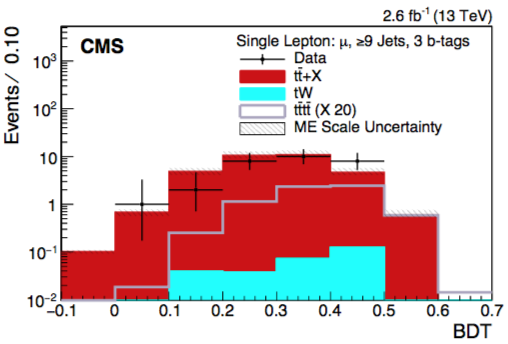
\includegraphics[scale=0.2]{semilepbdt.png}
		\caption{Single $\mu$ event level BDT in $\geq$9 jet 3 btag category}
	\end{figure}
	\column{0.5\textwidth} \center
	\begin{figure}
		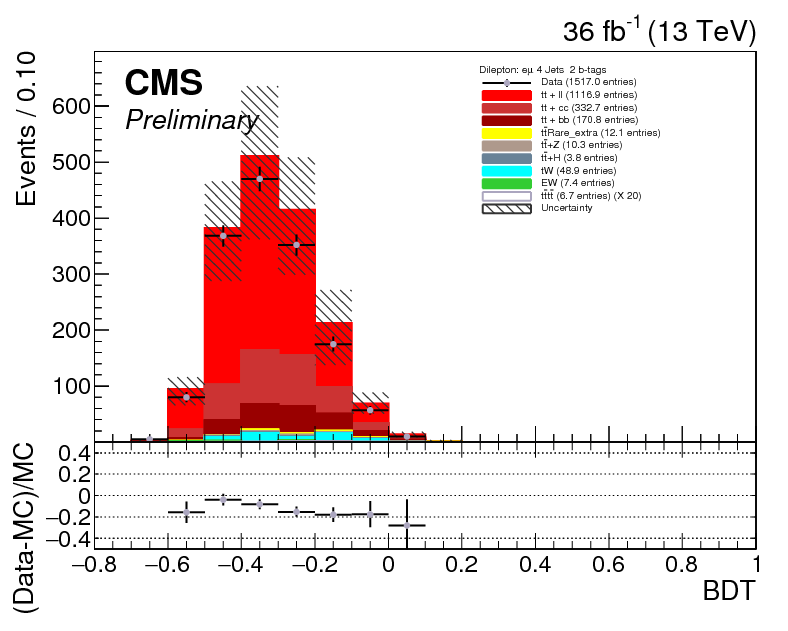
\includegraphics[scale=0.12]{dilepbdt.png}
		\caption{$\mu e$ event level BDT in CR}
	\end{figure}
\end{columns}
\bigskip
\textbf{Event categorization in $N_{j} \otimes N_{tags}^{M}$ for limit fitting}
\begin{itemize}
	\item{Single lepton channel}
	\begin{itemize}
		\item $\mu$: $N_{j}$: 7, 8, 9, 10+; $N_{tags}^{M}$: 2, 3, 4+
		\item $e$: $N_{j}$: 8, 9, 10+; $N_{tags}^{M}$: 2, 3, 4+
	\end{itemize}
	\item OS Dilepton channel: $N_{j}$: 4-5, 6-7, 8+; $N_{tags}^{M}$: 2, 3+
\end{itemize}
\end{frame}

%------------------------------------------------

\begin{frame}
\frametitle{Control Plots (BDT Input Variables)}
\begin{itemize}
	\item {\small Single lepton channel}
	{\tiny $BDT_{trijet2}, HTH, H_{T}^{b}, H_{T}^{Rat}, p_{T}^{5th jet}, p_{T}^{6th jet}, M_{RE}^{H}, HT_{X}, p_{T}^{lep}, CSV_{3}, CSV_{4}, CSV_{3rdjet}, CSV_{4thjet}$}
	\vspace{-12pt}
	\begin{columns}
		\column{0.25\textwidth} \begin{figure} 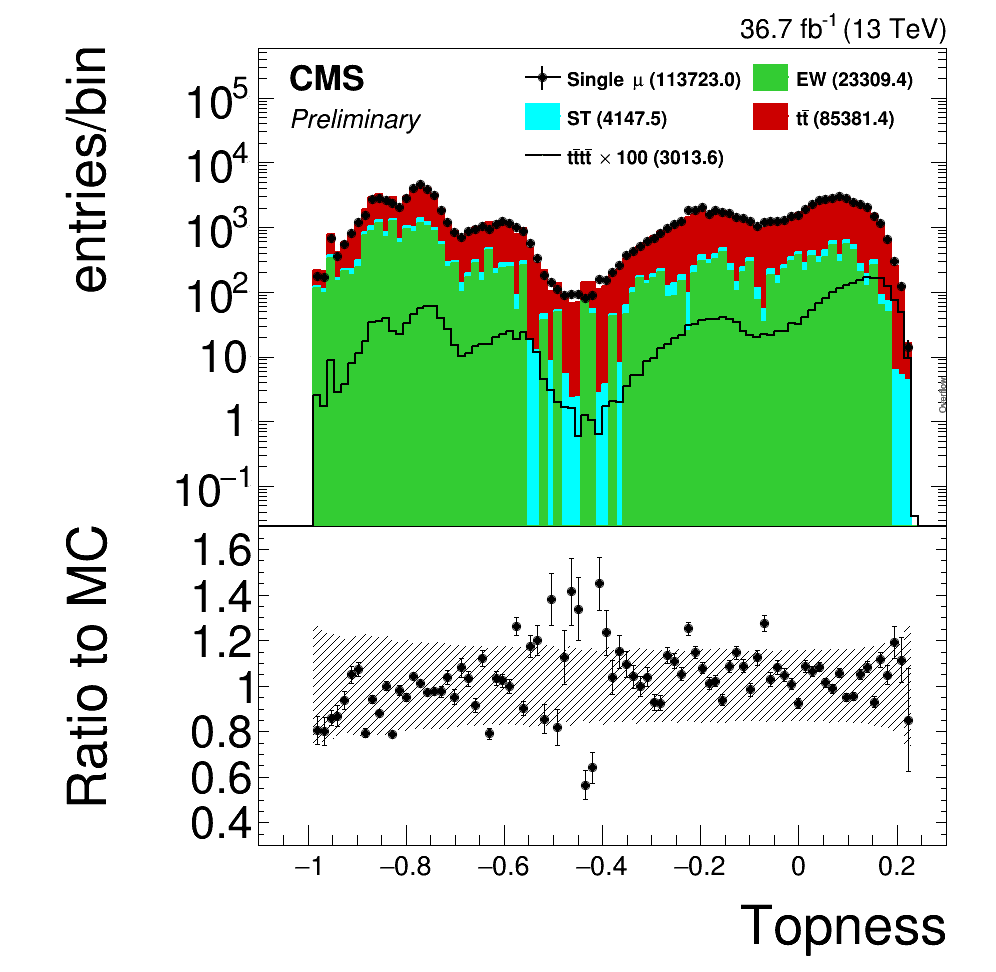
\includegraphics[scale=0.08]{multitopness.png} \end{figure}
		\column{0.25\textwidth} \begin{figure} 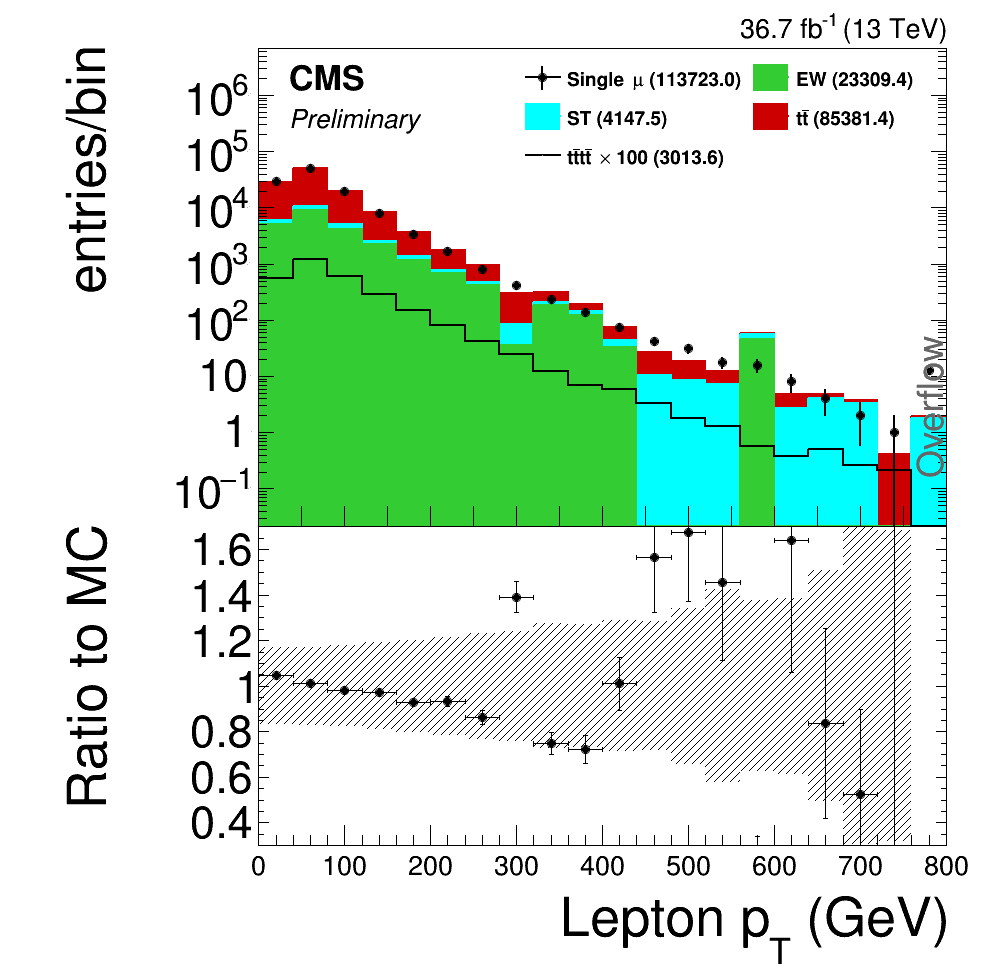
\includegraphics[scale=0.08]{leptonpt.png} \end{figure}
		\column{0.25\textwidth} \begin{figure} 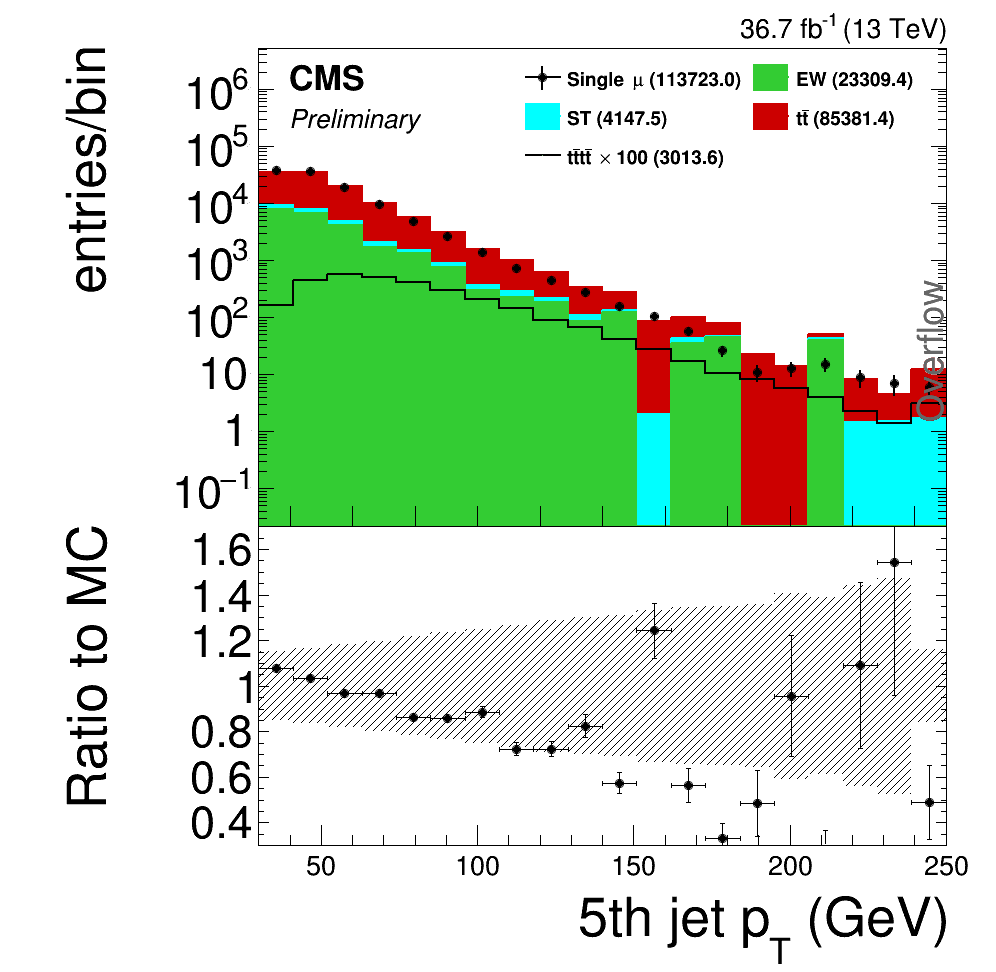
\includegraphics[scale=0.08]{5thjetpt.png} \end{figure}
		\column{0.25\textwidth} \begin{figure} 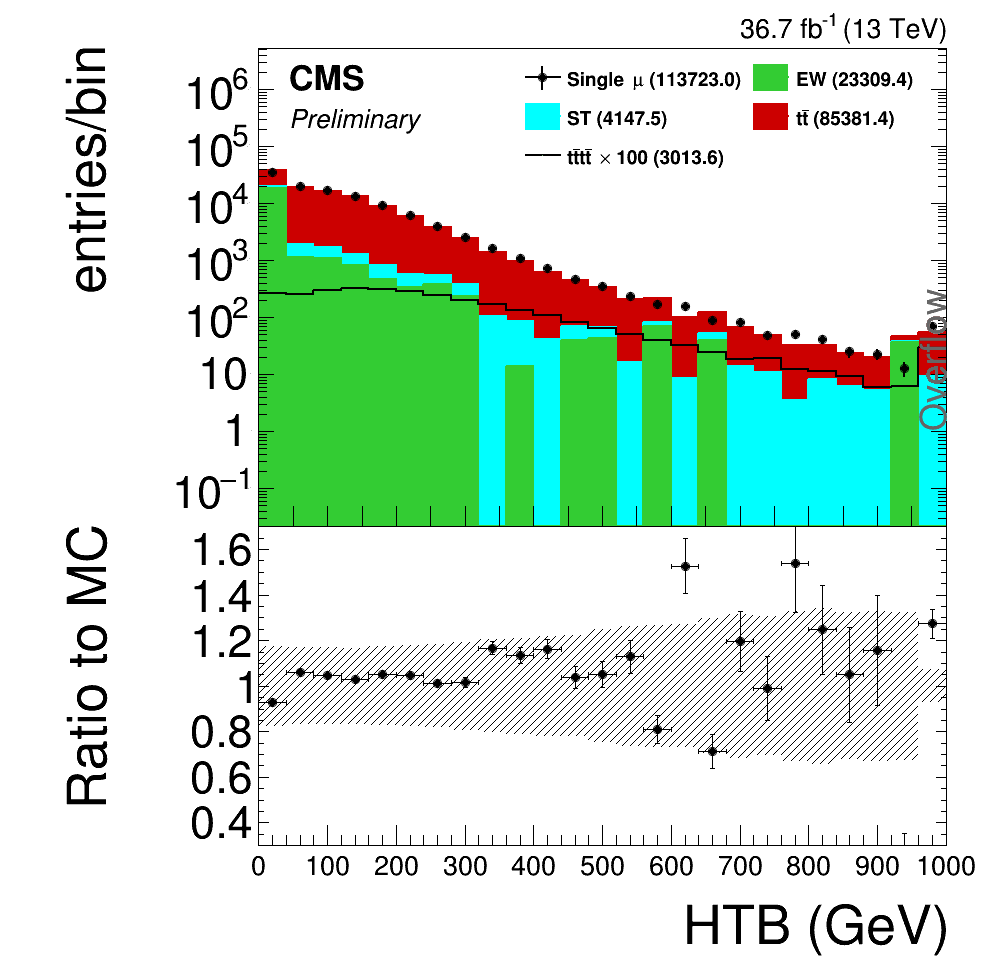
\includegraphics[scale=0.08]{HTB.png} \end{figure}
	\end{columns}
	\item {\small OS Dilepton channel}
	{\tiny $N_{j}, BDT_{trijet1}, H_{T}^{b}, H_{T}^{2M}, HTH, S, H_{T}^{Rat}, p_{T}^{l1}, \eta^{l1}, \Delta R_{ll}, \Delta R_{bb}, N_{tags}^{L}, N_{tags}^{M}, p_{T}^{3rd jet}, p_{T}^{4th jet}$}
	\vspace{-15pt}
	\begin{columns}
		\column{0.25\textwidth} \begin{figure} 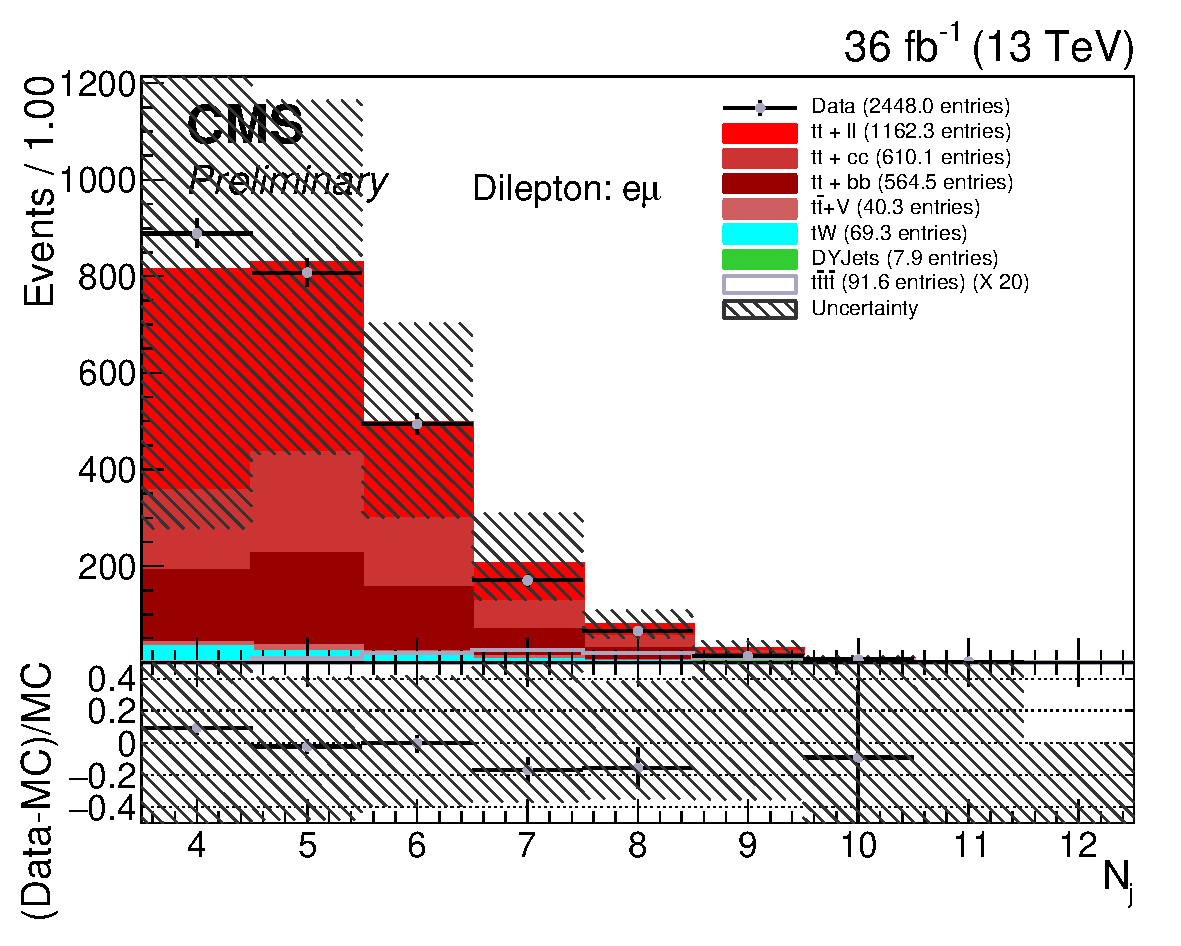
\includegraphics[scale=0.15]{njets_di.pdf} \end{figure}
		\column{0.25\textwidth} \begin{figure} 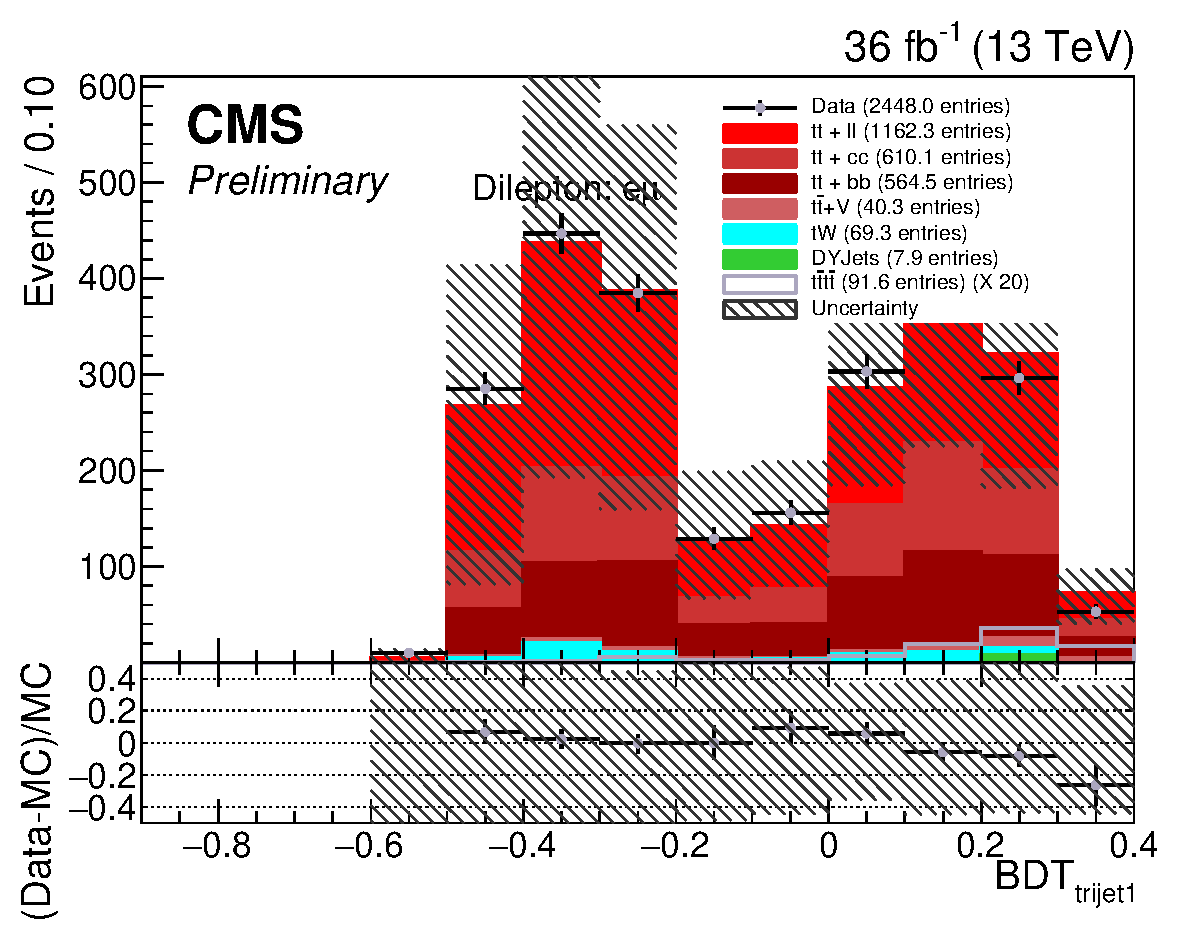
\includegraphics[scale=0.15]{topness_di.pdf} \end{figure}
		\column{0.25\textwidth} \begin{figure} 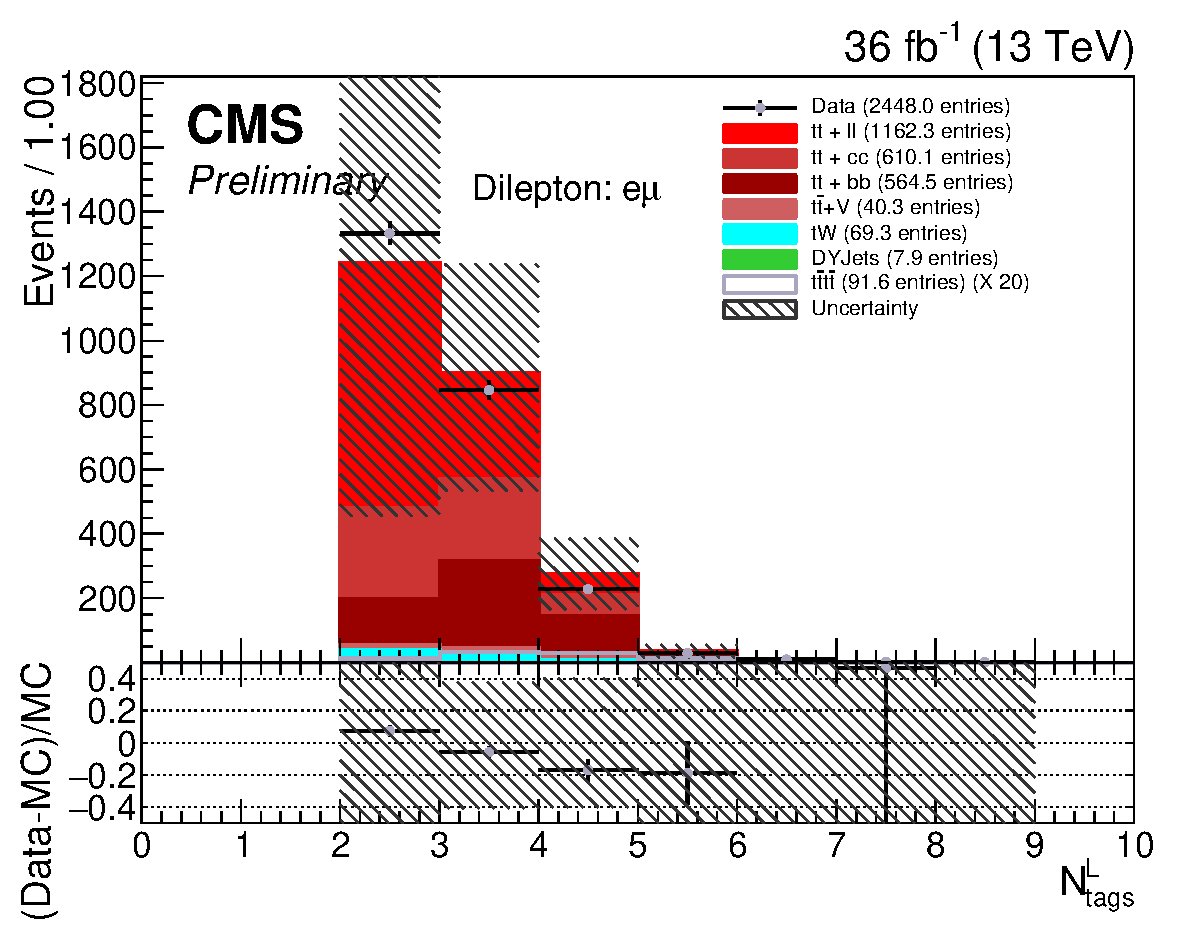
\includegraphics[scale=0.15]{nLtags_di.pdf} \end{figure}
		\column{0.25\textwidth} \begin{figure} 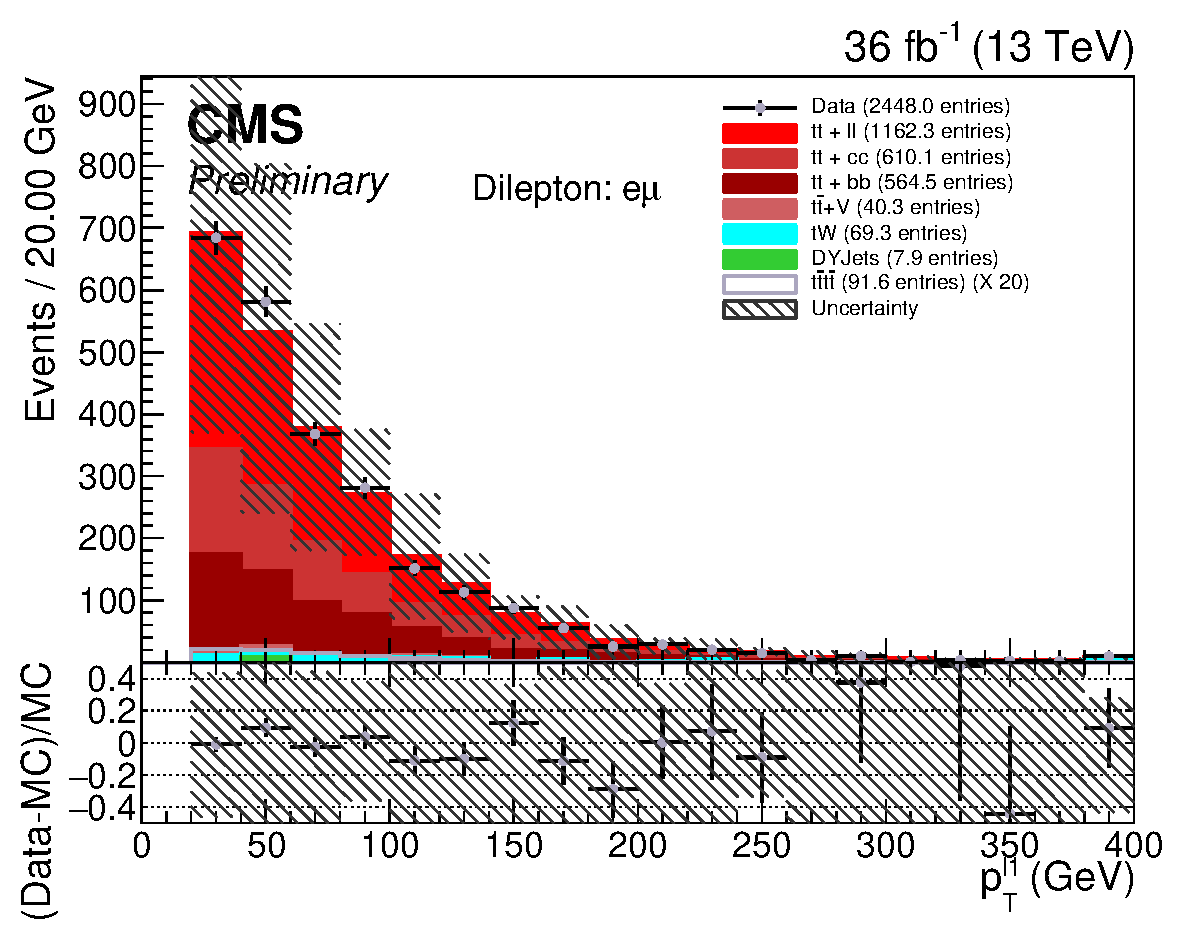
\includegraphics[scale=0.15]{l1pt_di.pdf} \end{figure}
	\end{columns}
	\item {\small Overall reasonable distributions agreement within uncertainties.}
\end{itemize}

\end{frame}

%------------------------------------------------

\begin{frame}
\frametitle{Sources of Systematic Uncertainties}
\begin{columns}
	\column{0.5\textwidth} \textbf{Experimental Uncertainties}
	\begin{itemize}
		\item Luminosity uncertainty
		\item Pileup $\pm 1 \sigma$
		\item Lepton SFs uncertainty
		\item JER $\pm 1 \sigma$
		\item JES(split) \begin{itemize}
			\item SubTotalPileUp
			\item SubTotalRelative
			\item SubTotalPt
			\item SubTotalScale
			\item Jet flavor \end{itemize}
		\item b-tag CSV $\pm 1 \sigma$
		\item Heavy flavor fraction
		\item Top $p_{T}$ reweight
		\item Jet normalization
	\end{itemize}
	\column{0.5\textwidth} \textbf{Theoretical Uncertainties}
	\begin{itemize}
		\item ME scale
		\item MC cross sections
		\item UE tune
		\item PS scale
		\item ME-PS matching
		\item PDF
	\end{itemize}
\end{columns}
\end{frame}

%------------------------------------------------

\begin{frame}
\frametitle{Fit Strategy}
\begin{itemize}
	\item Likelihood fit using Combine Tool
	\vspace{10pt}
	\item Event level BDT output discriminator distributions for fit is performed simultaneously in different $N_{j} \otimes N_{tags}^{M}$ categories.
	\vspace{10pt}
	\item Blind highest jet/tag multiplicity categories. \begin{itemize}
		\item single lepton: blind 10+ jets \& 3+ tags category
		\item OS dilepton: blind 8+ jets \& 3+ tags category\end{itemize}
	\vspace{10pt}
	\item Combine results from single lepton channel and OS dilepton channel.
\end{itemize}
\end{frame}

%------------------------------------------------

\begin{frame}
\frametitle{Template Fit in Single Lepton Channel}
\vspace{-10pt}
\begin{table}
{\tiny
\caption{Single lepton blinded fitting results}
\vspace{0pt} 
\begin{tabular}{| c | c | c | c |}
\hline
Channel	&Expected limit	&Expected xsec	&Expected \\
 & $\times \sigma_{t\bar{t}t\bar{t}}^{SM}$ &  $fb$ &significance \\
\hline
$e$			& $23.5^{+7.0}_{-6.5}$ & $216.2^{+64}_{-60}$ &  0.09\\
\hline
$\mu$		& $16.0^{+7.0}_{-4.7}$ & $147.2^{+64}_{-43}$ &  0.12 \\
\hline
combined	& $9.4^{+4.0}_{-2.7}$ & $86.5^{+37}_{-25}$ & 0.25 \\
\hline
\end{tabular} 
}
\end{table}

\underline{Postfit BDT distributions} \vspace{-10pt}
\begin{columns}
	\column{0.5\textwidth}
	\begin{figure}
		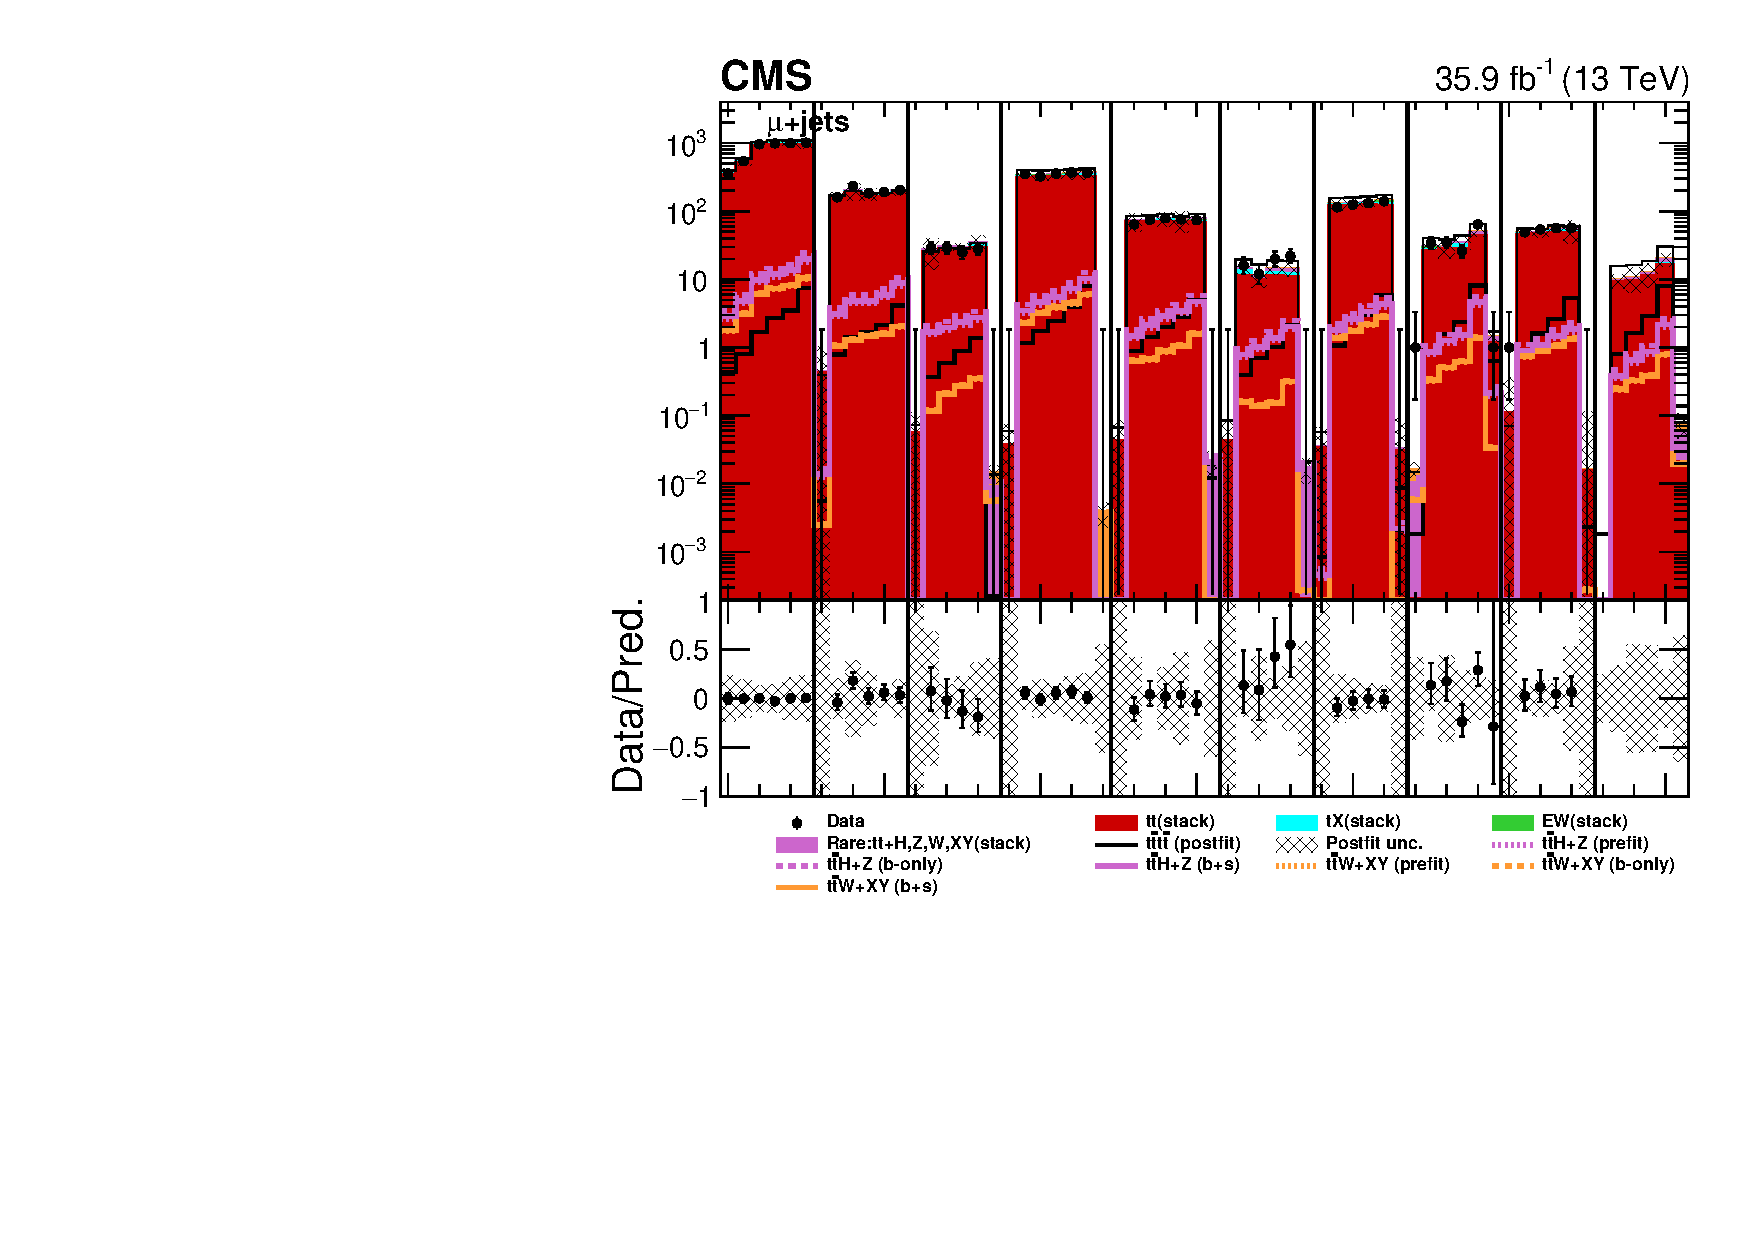
\includegraphics[width=\linewidth]{large_stat/mu/hist_muall_origbin_pub_lin}
	\end{figure}
	\column{0.5\textwidth}
	\begin{figure}
		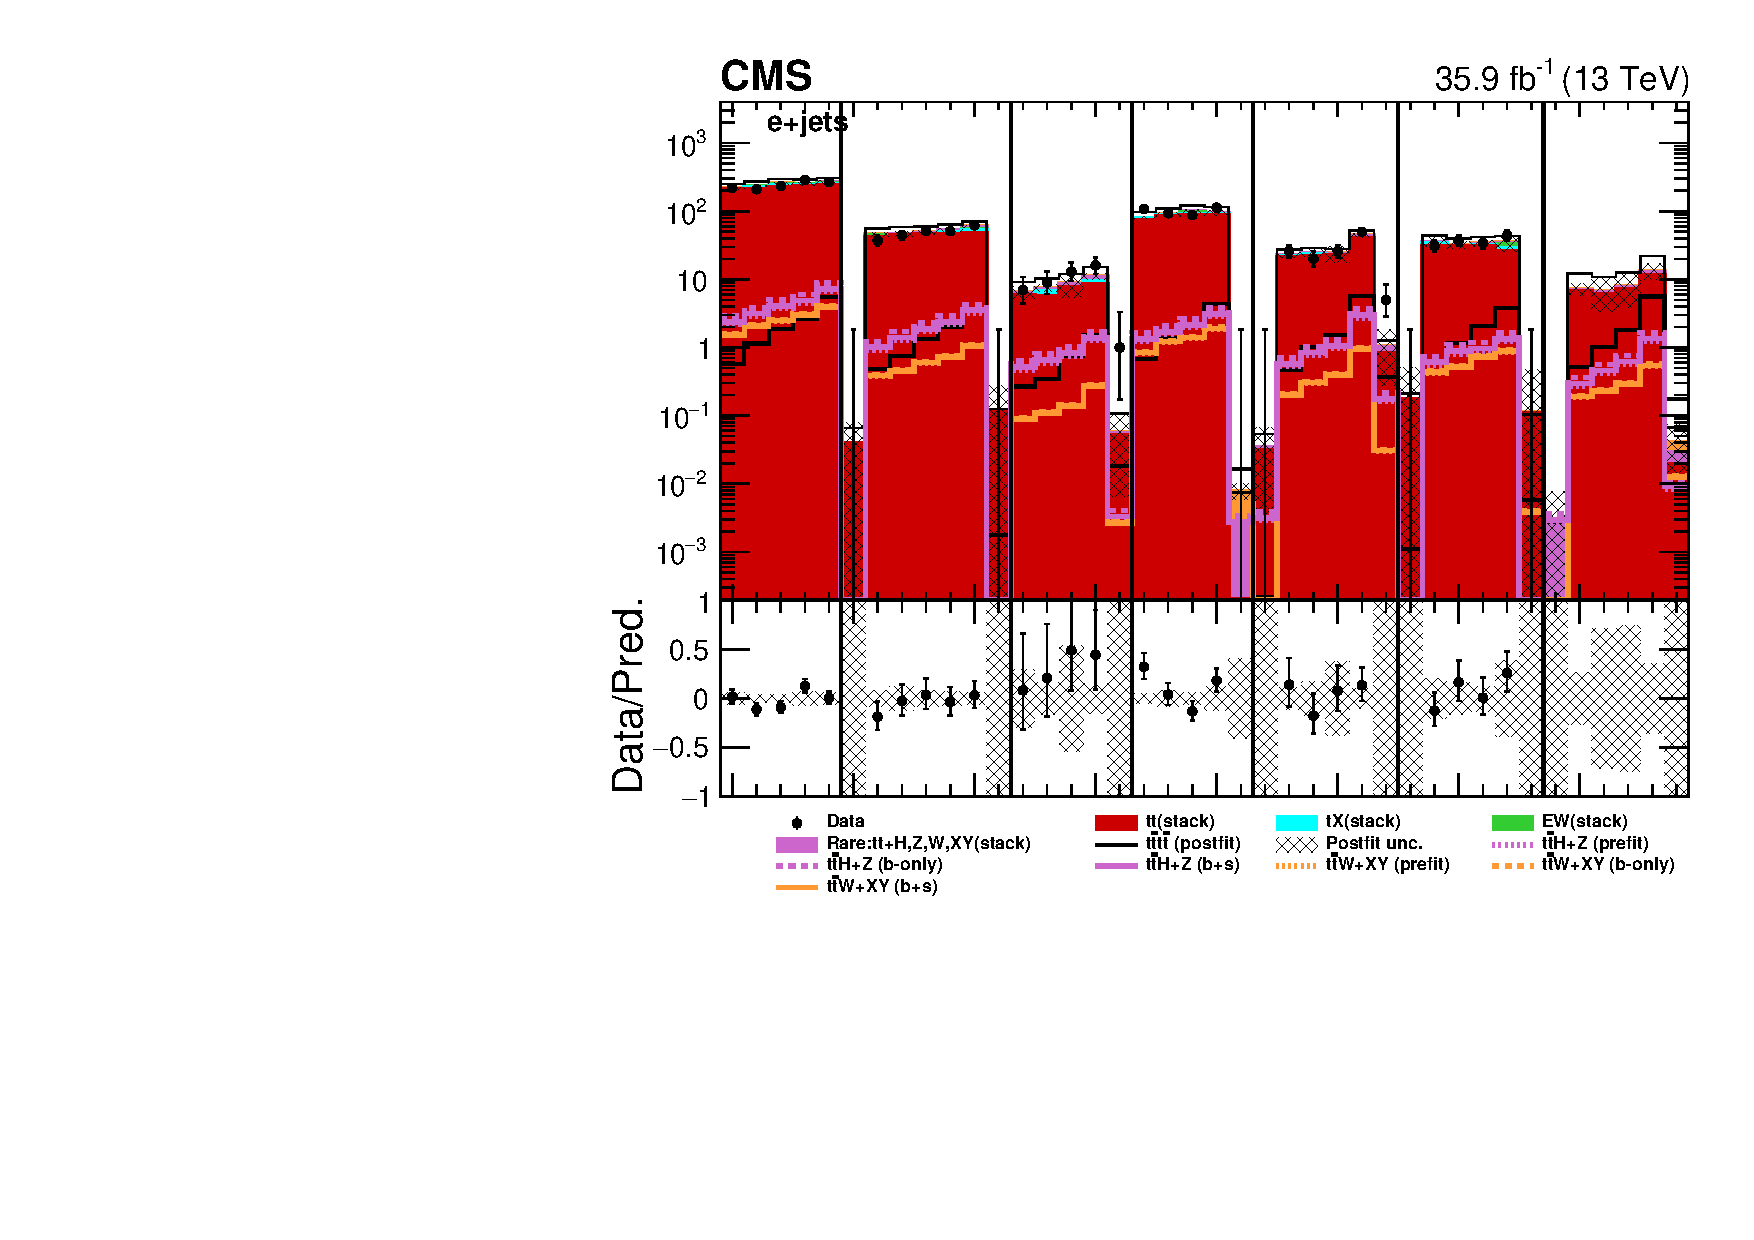
\includegraphics[width=\linewidth]{large_stat/el/hist_elall_origbin_pub_lin}
	\end{figure}
\end{columns}
	\begin{itemize}
	\item Equiprobable binning scheme
	\item Blind signal rich 10+/3+ category
	\item Reasonable description of the data in CRs
	\end{itemize}
\end{frame}

%------------------------------------------------

\begin{frame}
\frametitle{Fit Diagnostic in Single Lepton Channel}
\begin{columns}
\column{0.5\linewidth}
\begin{figure}
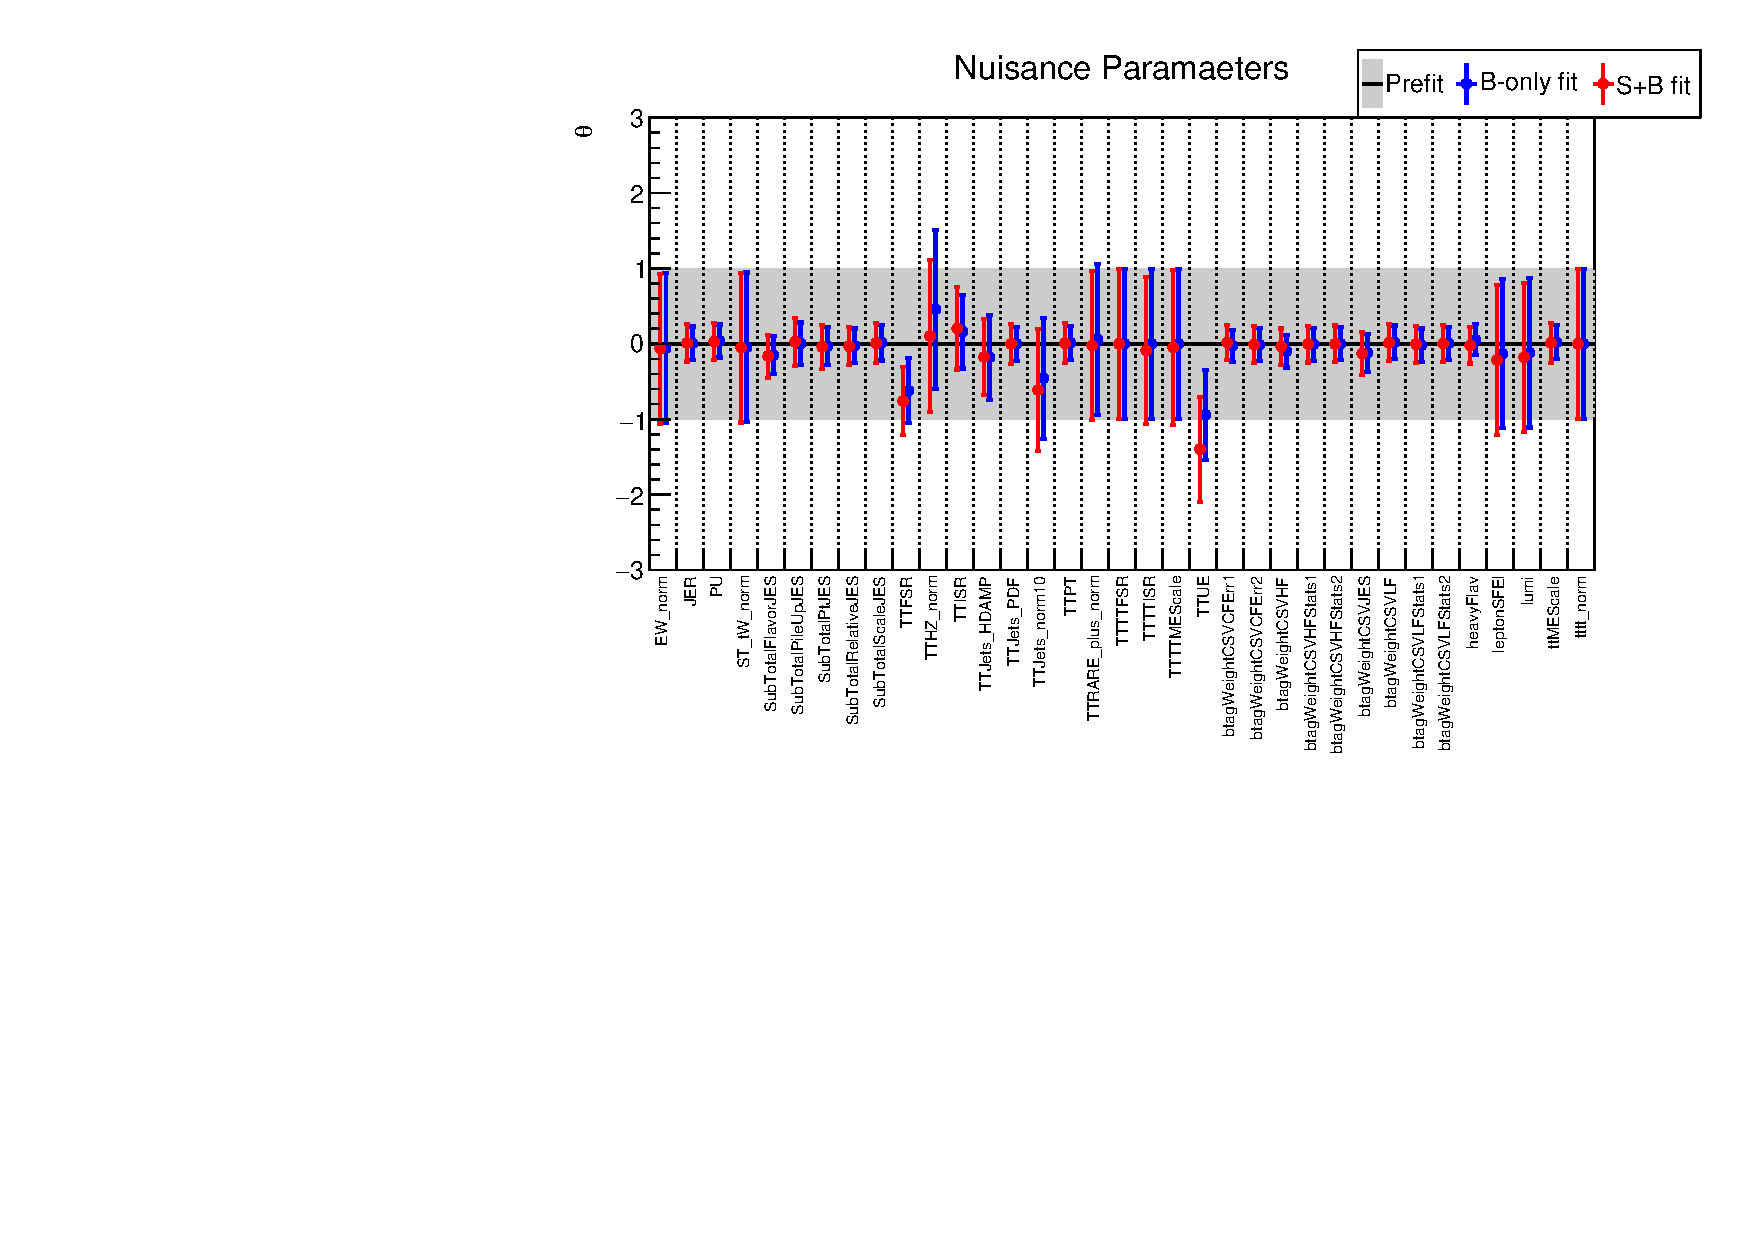
\includegraphics[width=\textwidth]{large_stat/mu/pulls}\caption{$\mu$+jets channel}
\end{figure}
\column{0.5\linewidth}
\begin{figure}
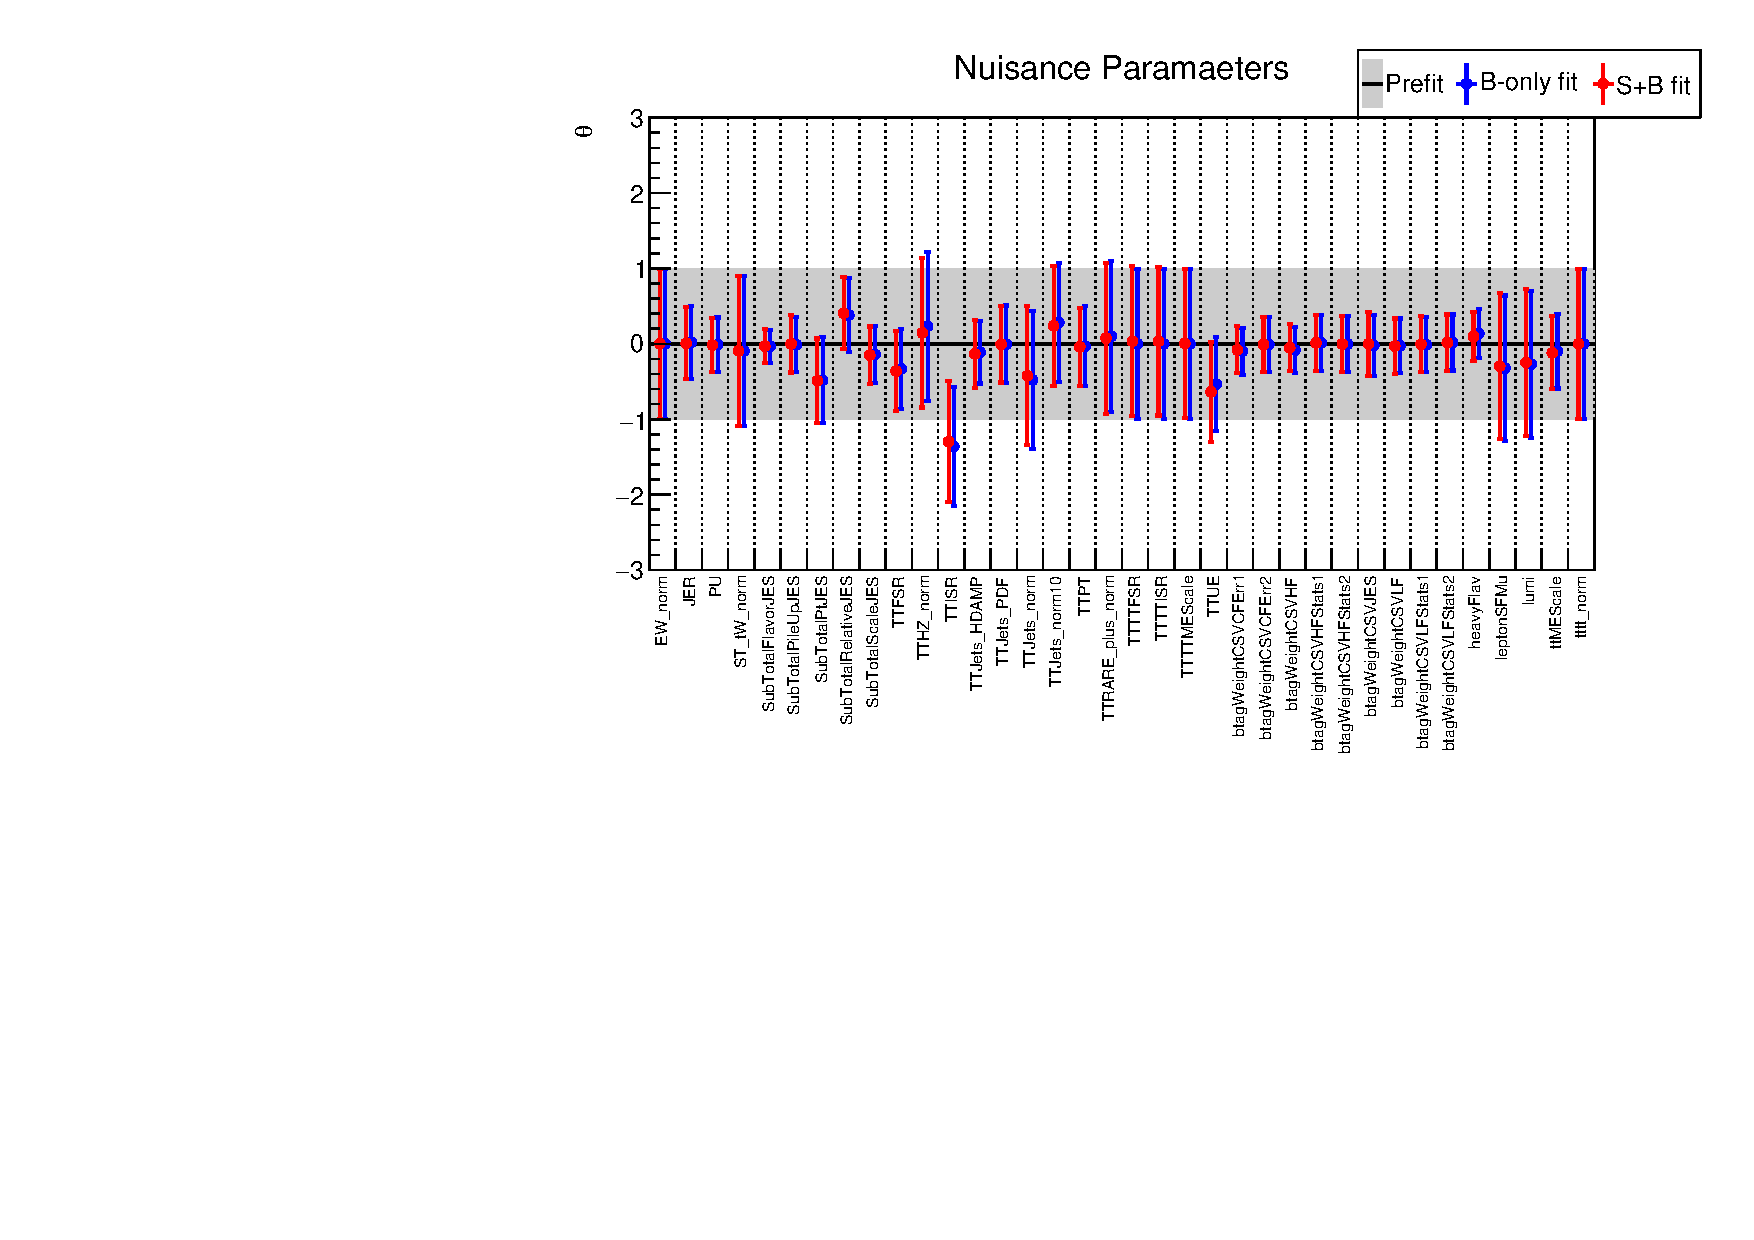
\includegraphics[width=\textwidth]{large_stat/el/pulls}\caption{$e$+jets channel}
\end{figure}
\end{columns}
	\begin{itemize}
	\item Post-fit uncertainty reduction is under investigation
	\end{itemize}
\end{frame}

%------------------------------------------------

\begin{frame}
\frametitle{Impact of Nuisance Parameters}
\begin{figure}
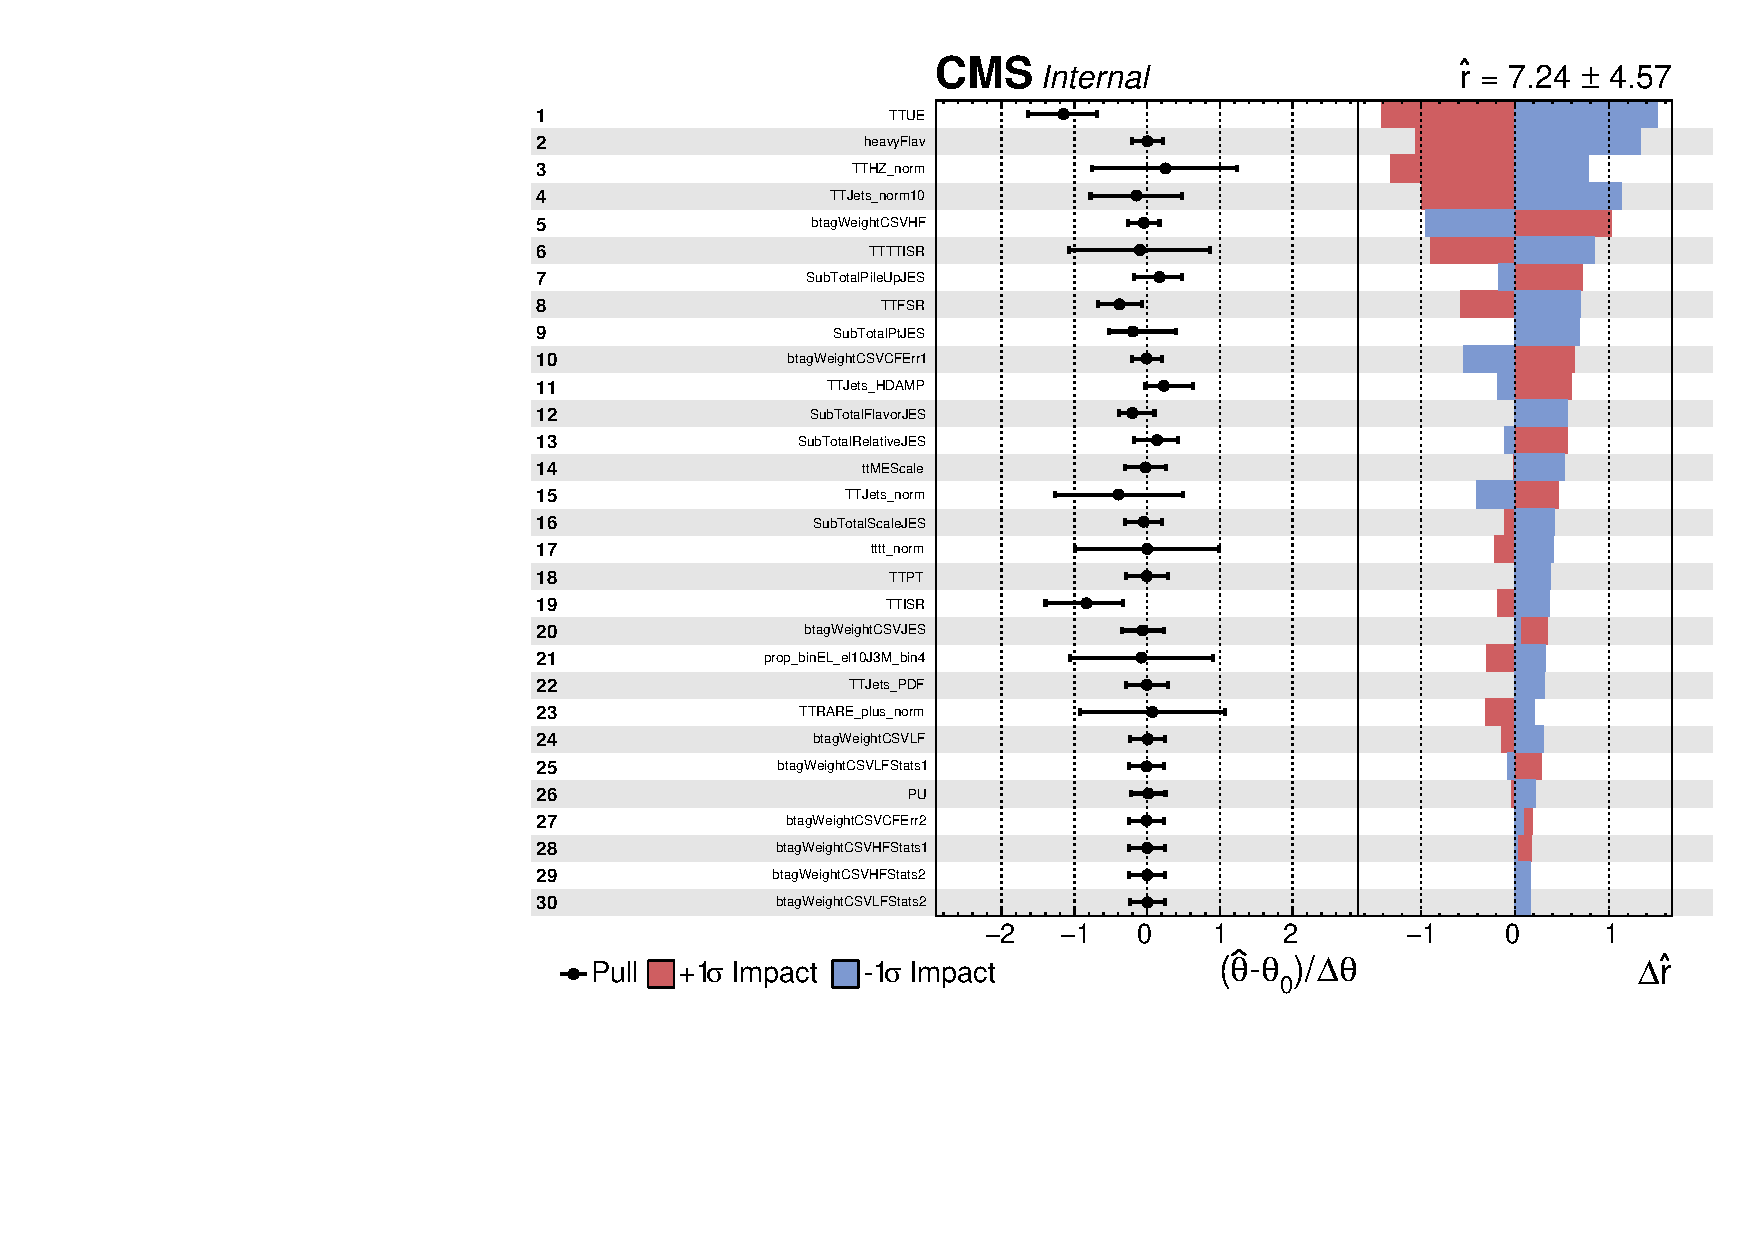
\includegraphics[width=0.5\textwidth]{large_stat/combo/pg_0001}
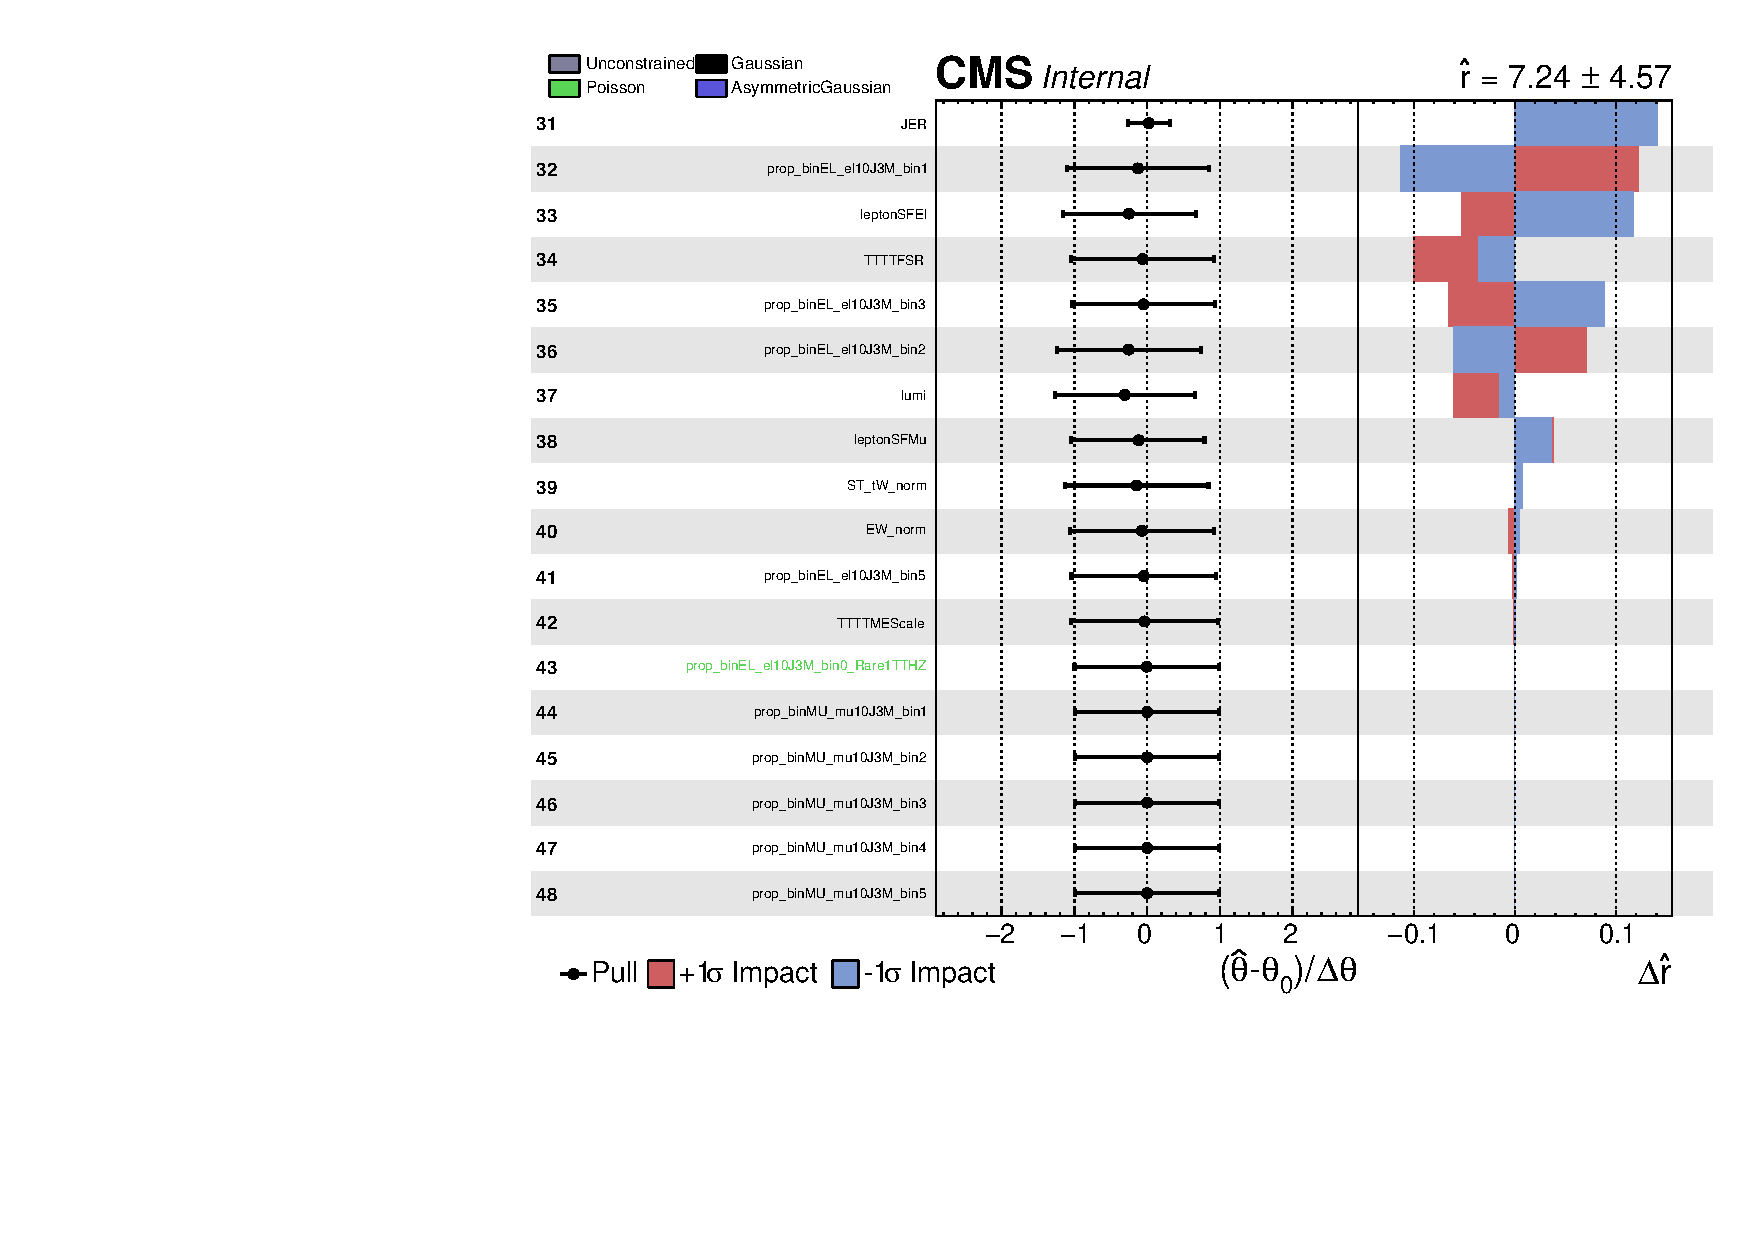
\includegraphics[width=0.5\textwidth]{large_stat/combo/pg_0002}
\end{figure}
\begin{itemize}
	\item Dominant sources of systematic uncertainty:
	\begin{itemize}
	\item UE variation. Affects jet multiplicity spectrum\\(Sample has low statistics)
	\item $t\bar{t}b\bar{b}$ normalization
	\item Normalization of $t\bar{t}Z,H \rightarrow b\bar{b}$
	\item Reweighting of HF component in CSV discriminant 
	\end{itemize}
\end{itemize}
\end{frame}

%------------------------------------------------

\begin{frame}
\frametitle{Template Fit in OS Dilepton Channel}
\vspace{-10pt} 
\begin{table}
\caption{OS dilepton blinded fitting results}
\vspace{0pt} 
\begin{tabular}{| c | c | c | c |}
\hline
Channel	&Expected limit	&Expected limit	&Expected \\
 & $\times \sigma_{t\bar{t}t\bar{t}}^{SM}$ &  $\times fb$ &significance \\
\hline
$\mu \mu$	&$14.56_{-5.24}^{+9.64}$ &$134_{-48}^{+89}$ &0.19  \\
\hline
$e \mu$		&$9.88_{-3.53}^{+6.53}$ &$91_{-32}^{+60}$ &0.37  \\
\hline
$ee$			&$17.56_{-6.19}^{+11.34}$ &$162_{-57}^{+104}$ &0.29  \\
\hline
combined		&$6.88_{-2.42}^{+4.44}$ &$63_{-22}^{+41}$ &0.52  \\
\hline
\end{tabular} 
\end{table}
\underline{Highest region blinded postfit BDT distributions} \vspace{-10pt}
\begin{columns}
	\column{0.33\textwidth}
	\begin{figure}
		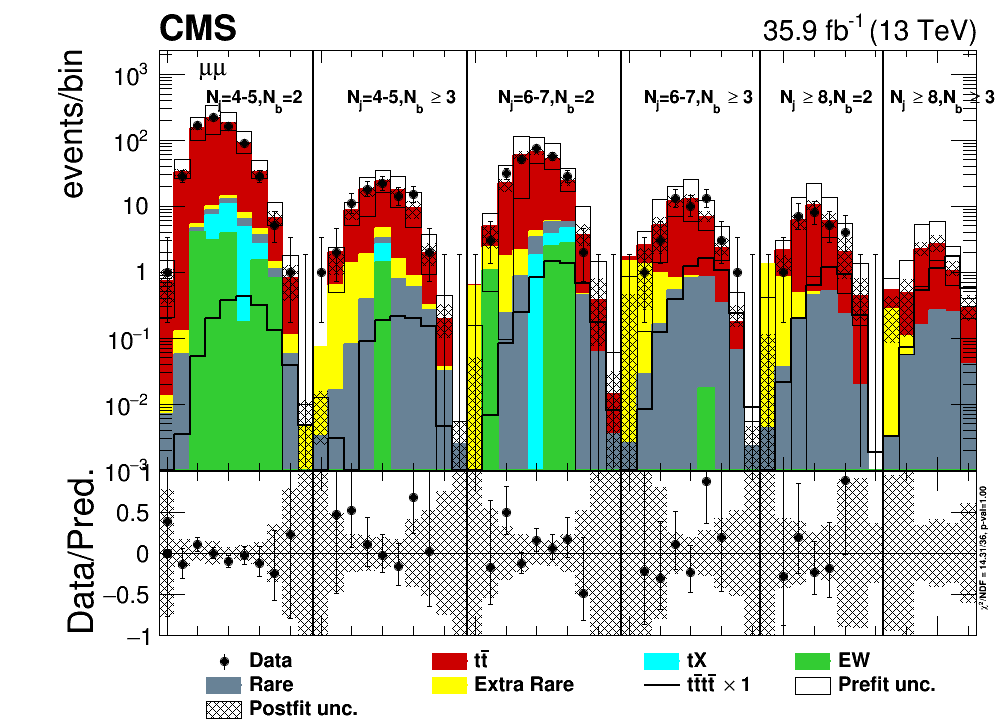
\includegraphics[width=\linewidth]{hist_mumu_log.png}
		\caption{$\mu \mu$ channel}
	\end{figure}
	\column{0.33\textwidth}
	\begin{figure}
		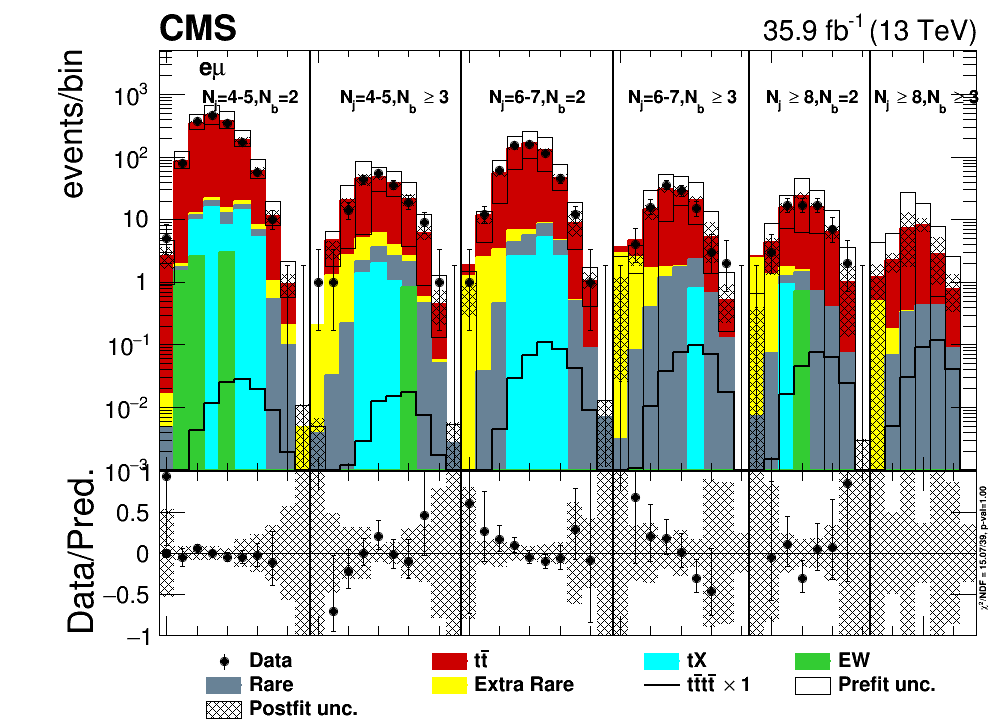
\includegraphics[width=\linewidth]{hist_muel_log.png}
		\caption{$e\mu$ channel}
	\end{figure}
	\column{0.33\textwidth} 
	\begin{figure}
		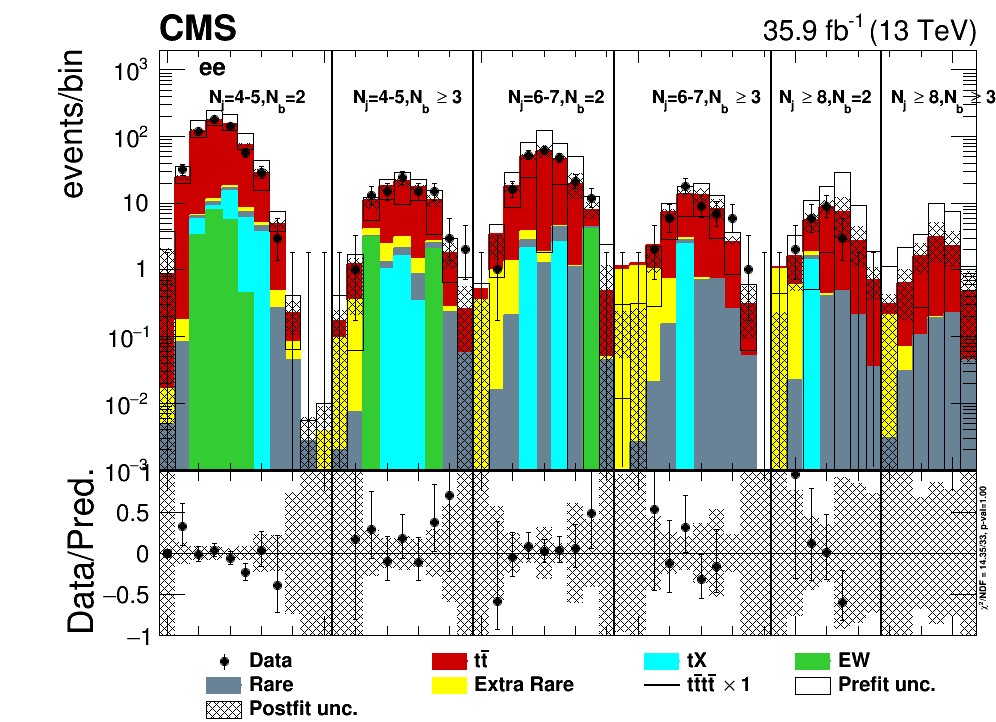
\includegraphics[width=\linewidth]{hist_elel_log.png}
		\caption{$ee$ channel}
	\end{figure}
\end{columns}
\end{frame}

%------------------------------------------------

\begin{frame}
\frametitle{Fit Diagnostic in OS Dilepton Channel}
\vspace{-10pt}
\begin{columns}
\column{0.5\textwidth}
	\begin{figure}
		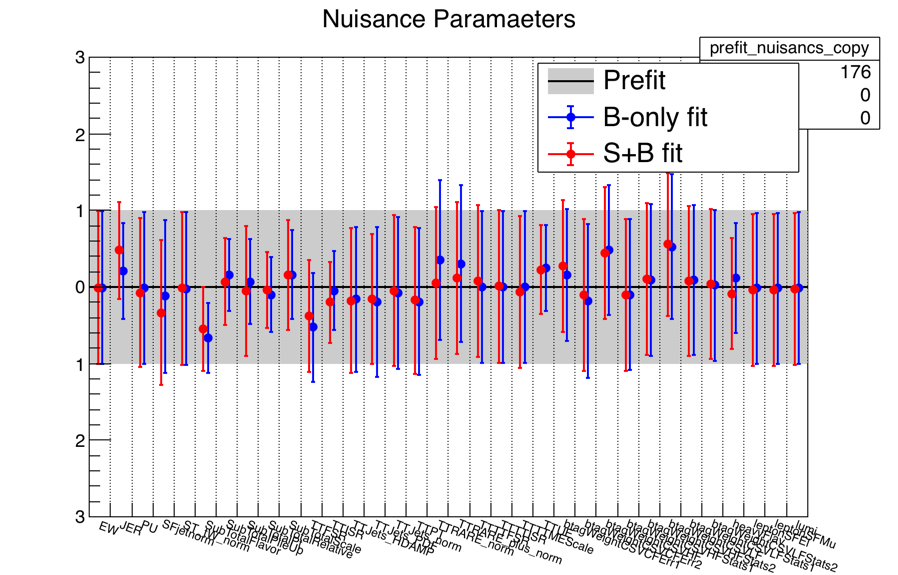
\includegraphics[scale=0.15]{mumuNP.png}
		\vspace{-10pt} \caption{nuisance pulls in $\mu \mu$}
	\end{figure}
	\vspace{-20pt}
	\begin{figure}
		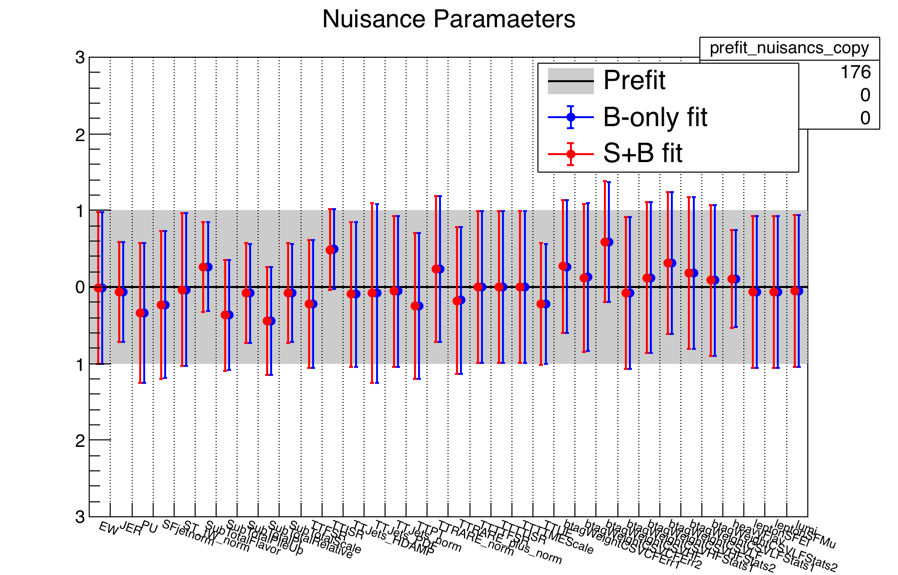
\includegraphics[scale=0.15]{muelNP.png}
		\vspace{-10pt} \caption{nuisance pulls in $e \mu$}
	\end{figure}
\column{0.5\textwidth}
	\begin{itemize}
		\item Most signal sensitive region is blinded
		\item No extreme pulls or constraints.
		\item Reasonable behavior for all the NPs
		\item Results are consistent between three sub-channels
	\end{itemize}
\end{columns}
\end{frame}

%------------------------------------------------

\begin{frame}
\frametitle{Fit Diagnostic in OS Dilepton Channel}
\vspace{-10pt}
\begin{columns}
\column{0.5\textwidth}
	\begin{figure}
		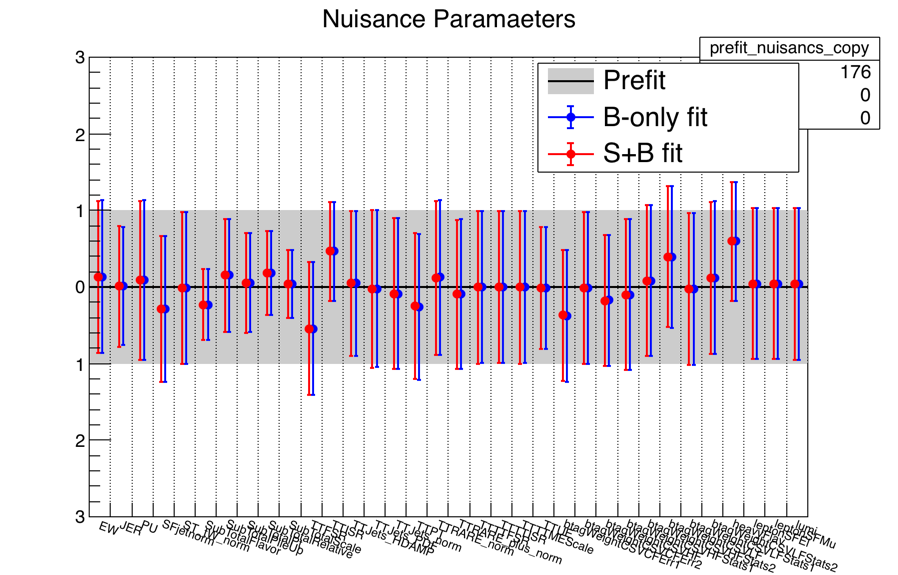
\includegraphics[scale=0.15]{elelNP.png}
		\vspace{-10pt} \caption{nuisance pulls in $ee$}
	\end{figure}
	\vspace{-20pt}
	\begin{figure}
		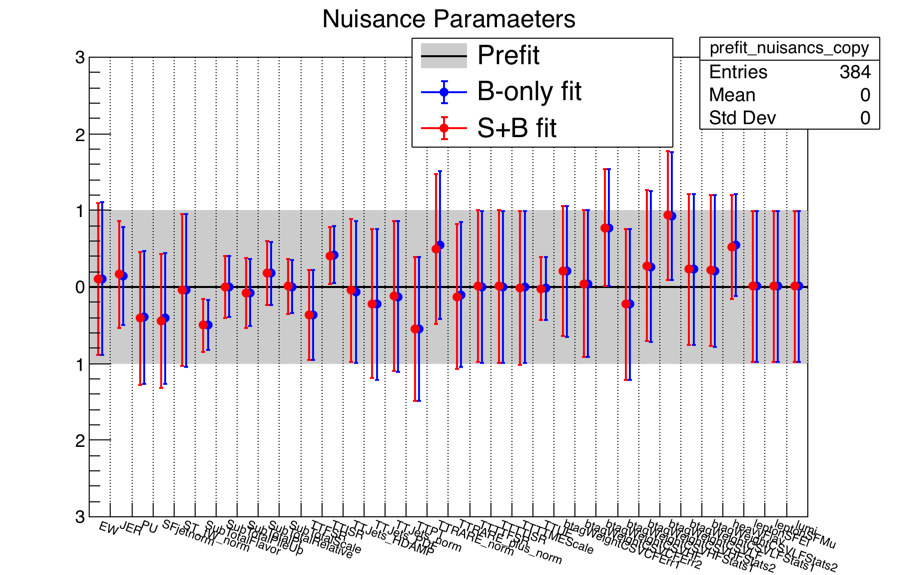
\includegraphics[scale=0.15]{combNP.png}
		\vspace{-10pt} \caption{nuisance pulls in OS dilep}
	\end{figure}
\column{0.5\textwidth}
	\begin{itemize}
		\item Mainly the sub-components of JES are constrained 
		\begin{itemize} 
			\item Statistic fluctuation
			\item Correlated with other NPs
		\end{itemize}
	\end{itemize}
\end{columns}
\end{frame}

%------------------------------------------------

\begin{frame}
\frametitle{Nuisance Parameters with highest impact in OS dilep combined fit}
\vspace{-5pt}
\begin{itemize}
	\item {\small Signal systematics and TTRare have the largest impacts, as we are very close to the expected signal strength.}
	\item {\small Jet energy scale uncertainties and MC stats in signal enriched bins dominate.}
	\item {\small All nuisance parameters behave reasonably.}
	\item {\small Full list of nuisance impacts are on backup slides~\ref{impacts1} to ~\ref{impacts2}}
\end{itemize}
\vspace{-5pt}
\begin{figure}
	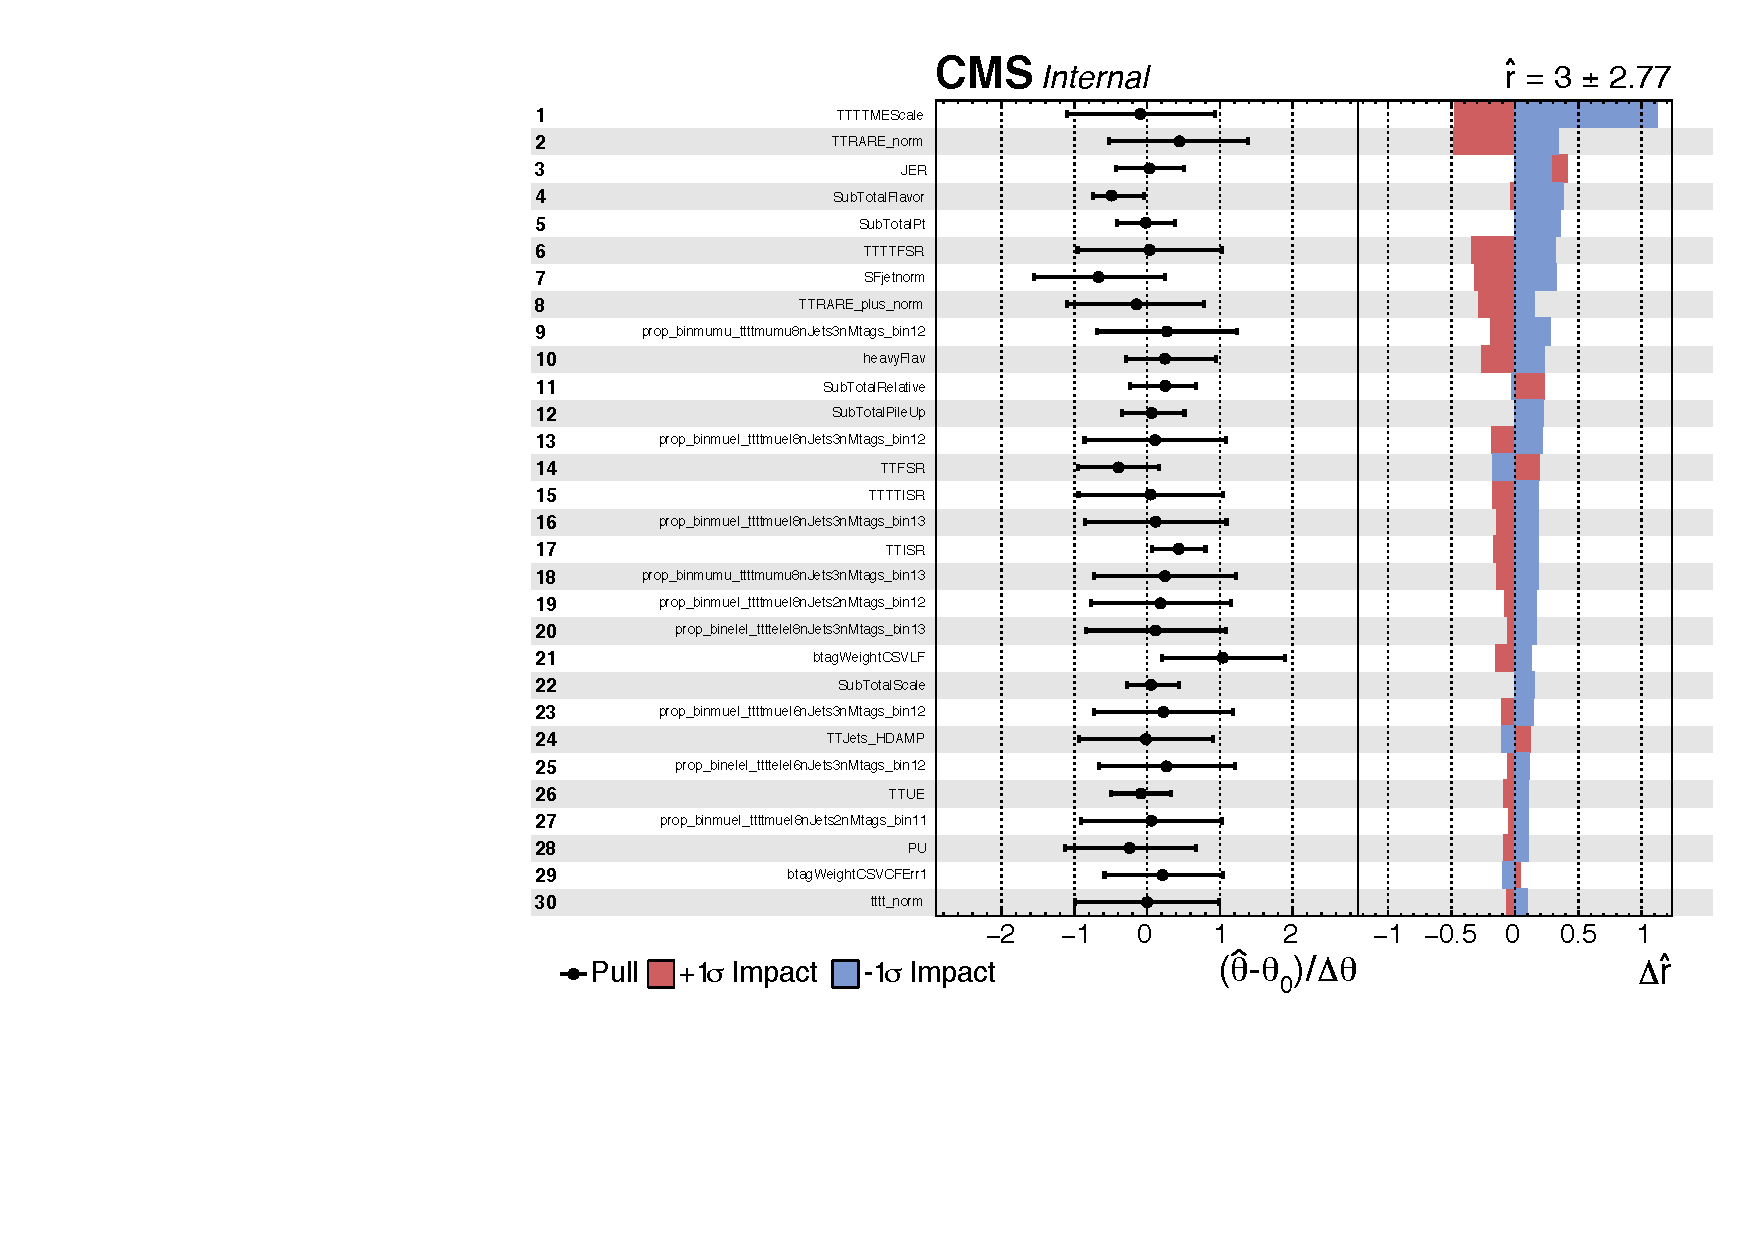
\includegraphics[width=0.5\textwidth]{impacts1.pdf}
	\vspace{-10pt} \caption{Impact of nuisance parameters on the parameter of interest}
\end{figure}
\end{frame}

%------------------------------------------------

\begin{frame}
\frametitle{Combined Results}

\begin{table}
\caption{Single lepton + OS dilepton blinded combined results}
\vspace{0pt} 
\begin{tabular}{| c | c | c | c |}
\hline
Channel	&Expected limit	&Expected limit	&Expected \\
 & $\times \sigma_{t\bar{t}t\bar{t}}^{SM}$ &  $\times fb$ &significance \\
\hline
l+jets	& $9.4^{+4.0}_{-2.7}$ & $86.5^{+37}_{-25}$ & 0.25 \\
\hline
OS ll+jets		&$6.9_{-2.4}^{+4.4}$ &$63_{-22}^{+41}$ & 0.52  \\
\hline
combined &$5.2_{-1.7}^{+2.6}$ &$48_{-16}^{+24}$ & 0.58 \\
\hline
\end{tabular} 
\end{table}
\begin{itemize}
\item Signal sensitivity is driven by the OS $ll+$jets channel
\end{itemize}
\end{frame}

%------------------------------------------------

\begin{frame}
\frametitle{Conslusion}
\underline{Current status:}
\begin{itemize}
\item Analysis blinded in order to optimize search regions/binning taking into account limited MC statistics
\item Expecting $\times 10$ more $t\bar{t}$ background MC with dedicated filters in signal rich search regions that have large statistical uncertainty
\begin{itemize}
\item New high jet multiplicity, high-$H_T$ filter was optimized for the analysis
\item MC requests are added to the system
\end{itemize}
\end{itemize}
\underline{Plans for coming weeks:}
\begin{itemize}
\item Finalize QCD background estimation
\item Include new MC samples when they are ready
\item Update ANs and paper draft 
\end{itemize}
%\begin{figure}
%\includegraphics[width=0.8\linewidth]{test}
%\end{figure}
\end{frame}

%------------------------------------------------



%------------------------------------------------

\begin{frame}
\center
{\huge Backups}
\end{frame}

%------------------------------------------------

\begin{frame}[label=newsample]
\frametitle{Filter optimized for l+jets channel}
\begin{itemize}
\item{\footnotesize  Preferred configuration: $HT>500,\, \mathrm{nJets+nLep}\geq9,\, \mathrm{nLep}=1$ (9M)}
\end{itemize}
\begin{center}
{\tiny \begin{tabular}{|c|c|c|c|c|}
            \cline{1-5}
             & & \multicolumn{3}{|c|}{Acceptance loss in different jet multiplicity regions\footnote{Fraction of events passing offline cuts but rejected by gen filter}}\\
            \cline{1-5}
\hline Filter cuts & Filter eff. & SL ($N_J^{rec}=9$)& SL ($N_J^{rec}>9$)&  Ext ($\times 10$) \\  
\hline \thead{HT$>$500 \\  nJets+nLep $\geq$8 \\  $1$ lepton} & $0.005 \pm 0.0002$  & 0.11 & 0.08 & 21.8 M\\ 
\hline \rowcolor{lightgray}\thead{HT $>$ 500 \\  nJets+nLep $\geq\phantom{M}$9 \\  $1$ lepton} & $0.002 \pm 0.0001$  & 0.19 & 0.10 & 8.7M\\
\hline \thead{HT$>$500 \\  nJets+nLep$>$=10 \\  $1$ lepton} & $0.0007 \pm 6.5\times 10^{-5}$  & --- & 0.19 & 3M\\
\hline 
\end{tabular} }
\end{center}
\end{frame}

%------------------------------------------------

\begin{frame}
\frametitle{Filter optimized for OS dilpeton channel}
\begin{itemize}
\item{\footnotesize  Preferred configuration: $HT>500,\, \mathrm{nJets+nLep}\geq7,\,  \mathrm{nLep}=2$ (9M)}
\end{itemize}
\begin{center}
{\tiny \begin{tabular}{|c|c|c|c|c|}
            \cline{1-5}
             & & \multicolumn{3}{|c|}{Acceptance loss in different jet multiplicity regions\footnote{Fraction of events passing offline cuts but rejected by gen filter}}\\
            \cline{1-5}
\hline Filter cuts      & Filter eff.   & OS  ($N_J^{rec}=7$)& OS ($N_J^{rec}\geq8$)&  Ext ($\times 10$) \\
\hline \thead{HT$>$500 \\  nJets+nLep$>$=5 \\  $2$ lepton} & $0.0046 \pm 5.5e-05$  & 0.21 & 0.23 & 20 M\\
\hline \thead{HT$>$500 \\  nJets+nLep$>$=6 \\  $2$ lepton} & $0.0033 \pm 4.7e-05$  & 0.21 & 0.23 & 14.4 M\\
\hline \rowcolor{lightgray} \thead{HT$>$500 \\  nJets+nLep$>$=7 \\  $2$ lepton} & $0.0020 \pm 3.6e-05$  & 0.23 & 0.24 & 8.7 M\\
\hline \thead{HT$>$500 \\  nJets+nLep$>$=8 \\  $2$ lepton} & $0.0009 \pm 2.4e-05$  & 0.31 & 0.25 & 3.9 M\\
\hline
\end{tabular} }
\end{center}

\end{frame}

%------------------------------------------------

\begin{frame}[label=impacts1]
\frametitle{impacts of nuisance parameters}
\vspace{-10pt}
\begin{columns}
	\column{0.5\textwidth}
	\begin{figure}
		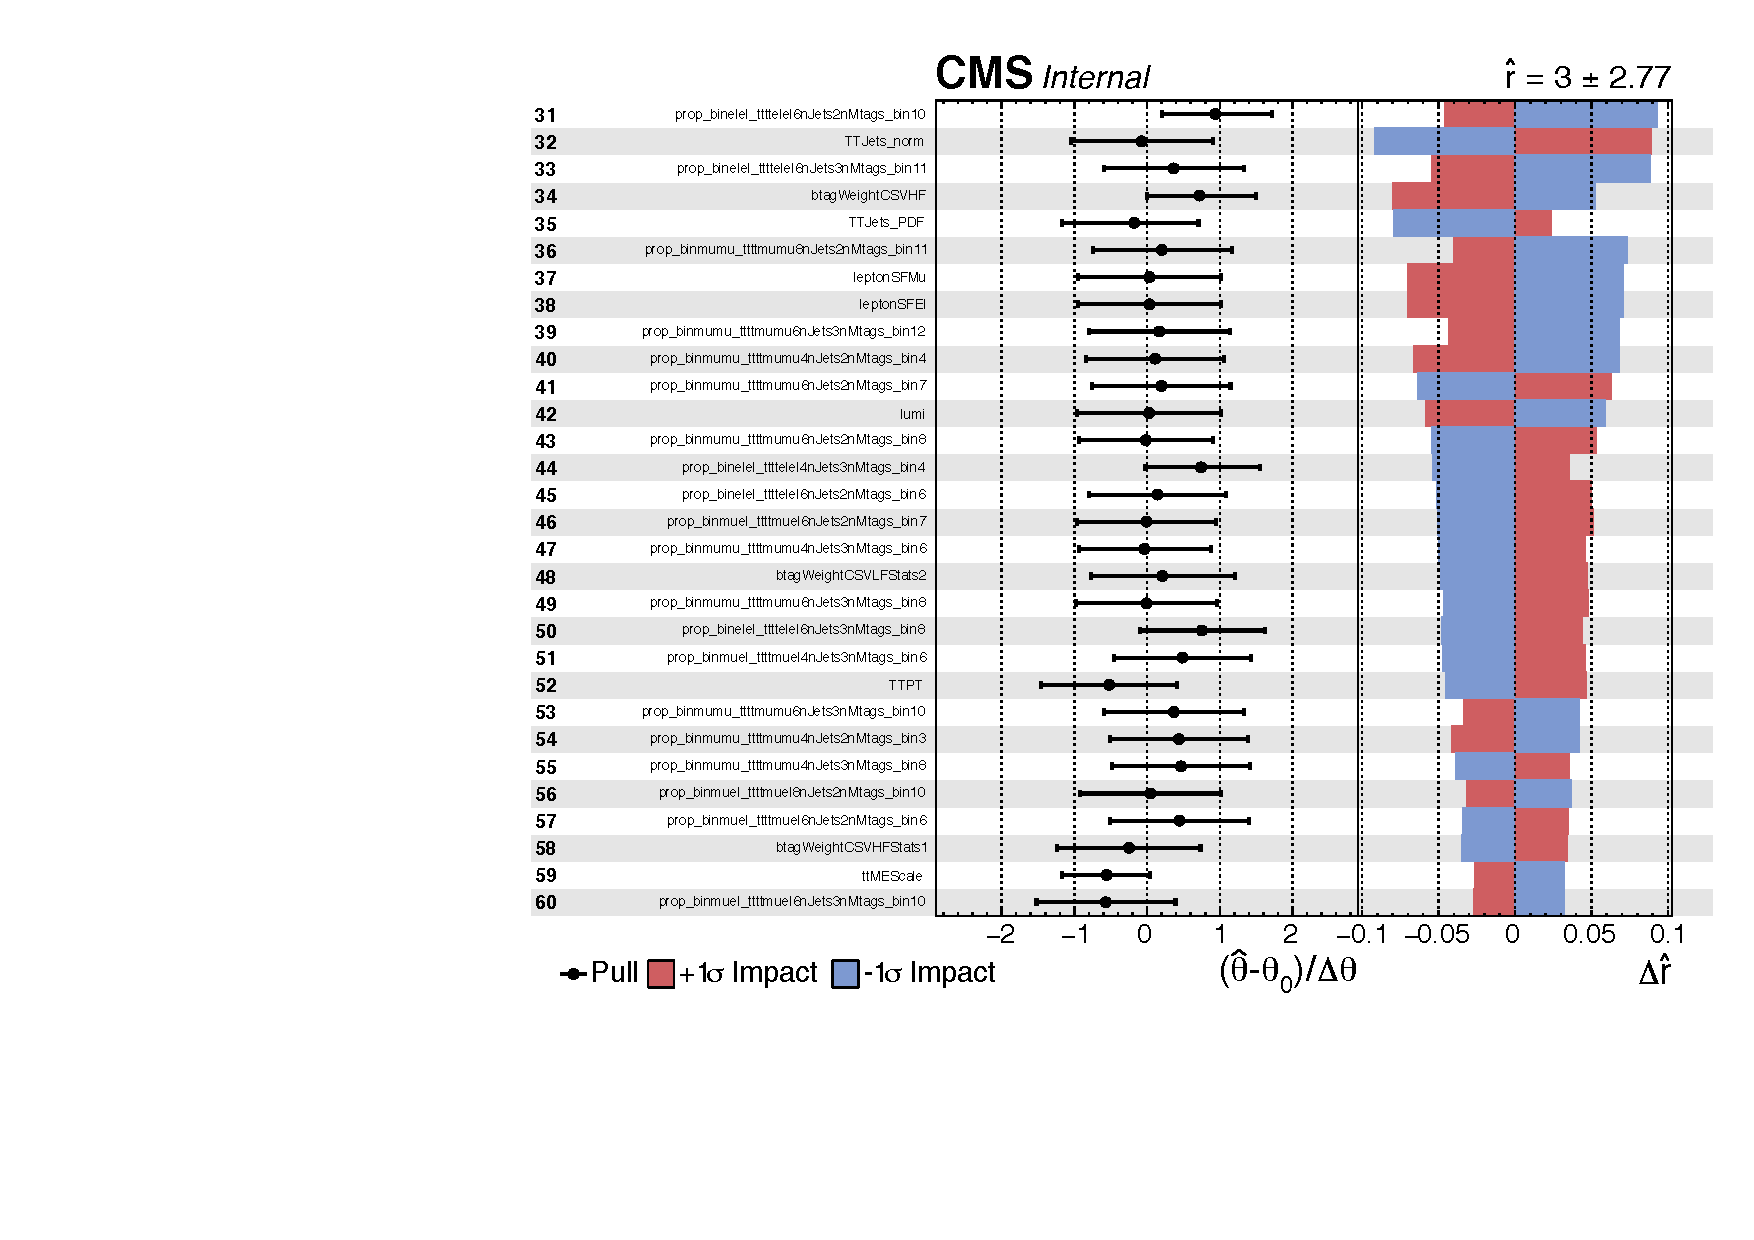
\includegraphics[width=0.9\textwidth]{impacts2.pdf}
	\end{figure}
	\column{0.5\textwidth}
	\begin{figure}
		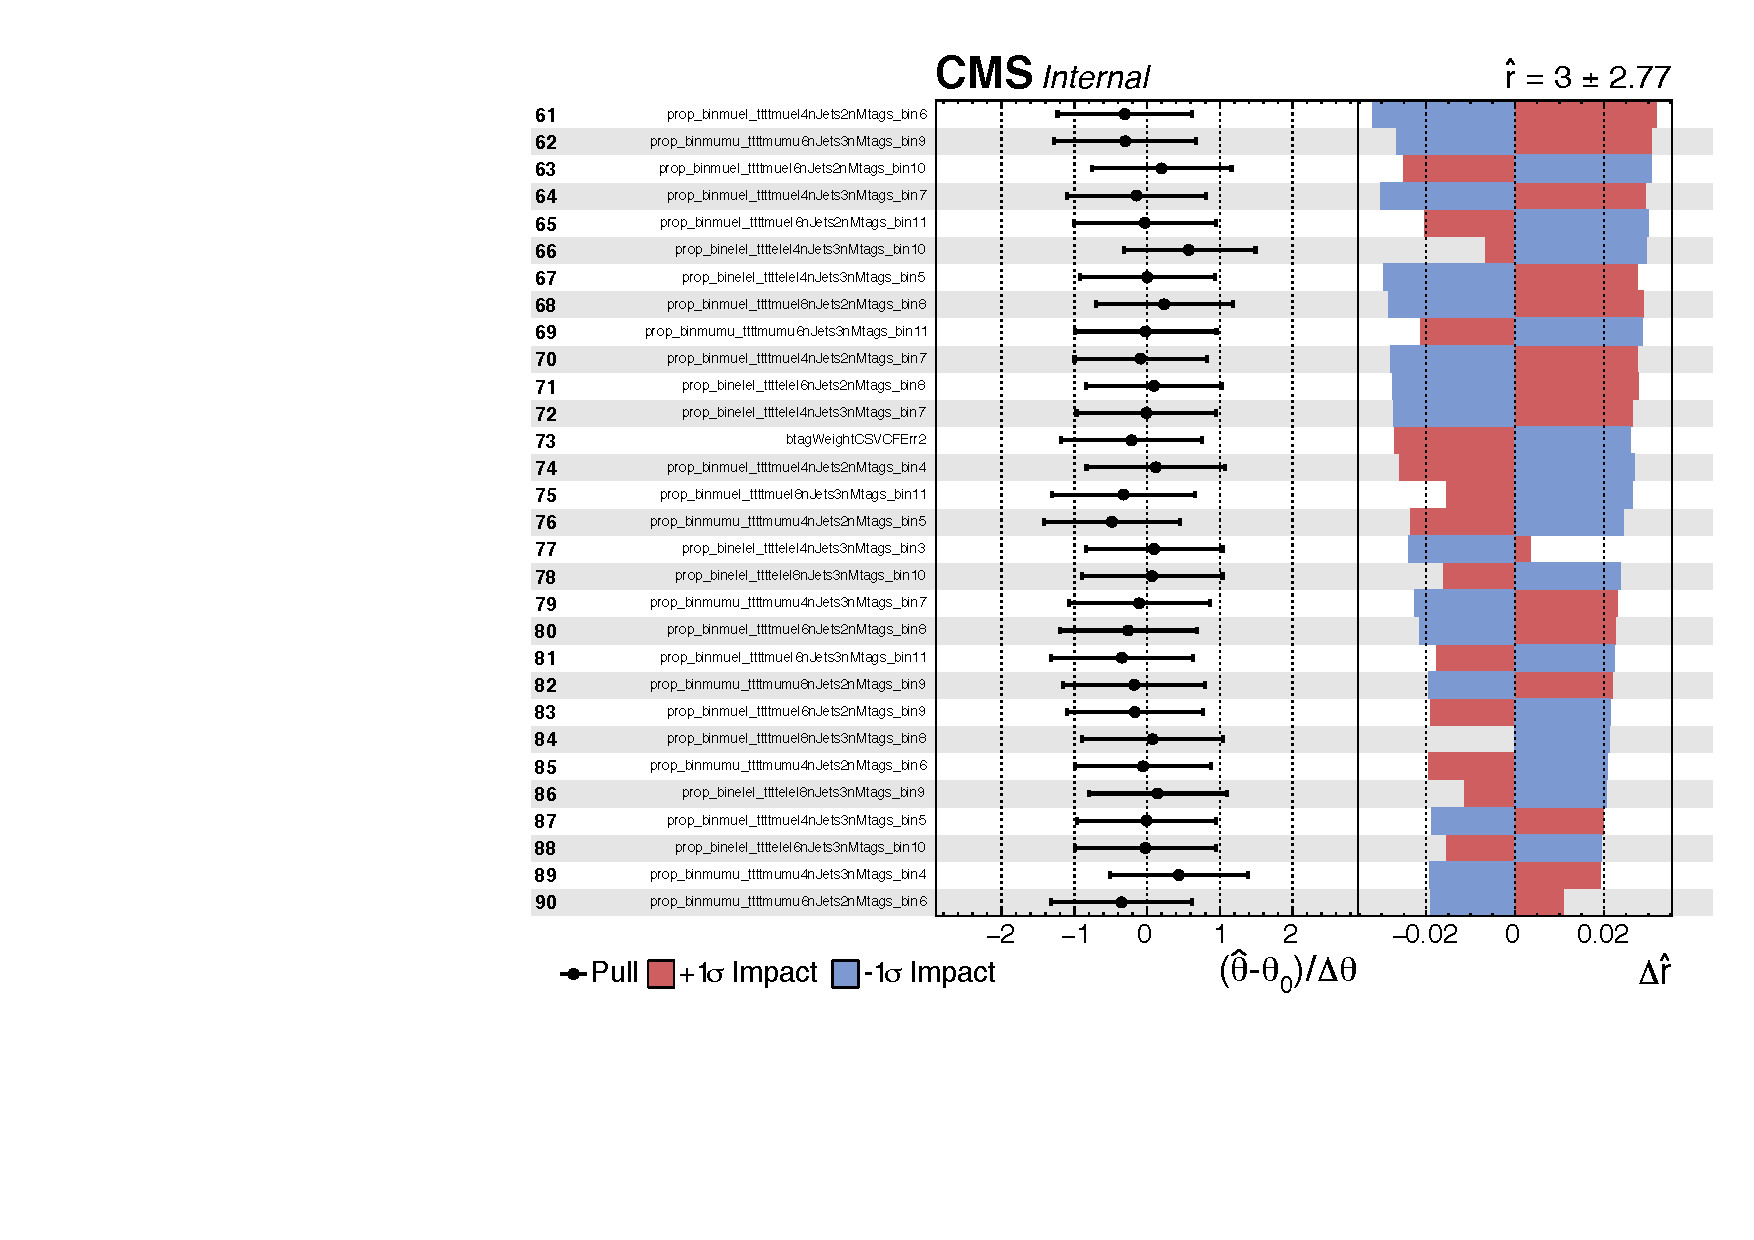
\includegraphics[width=0.9\textwidth]{impacts3.pdf}
	\end{figure}
\end{columns}
\vspace{-10pt}
\begin{figure}
	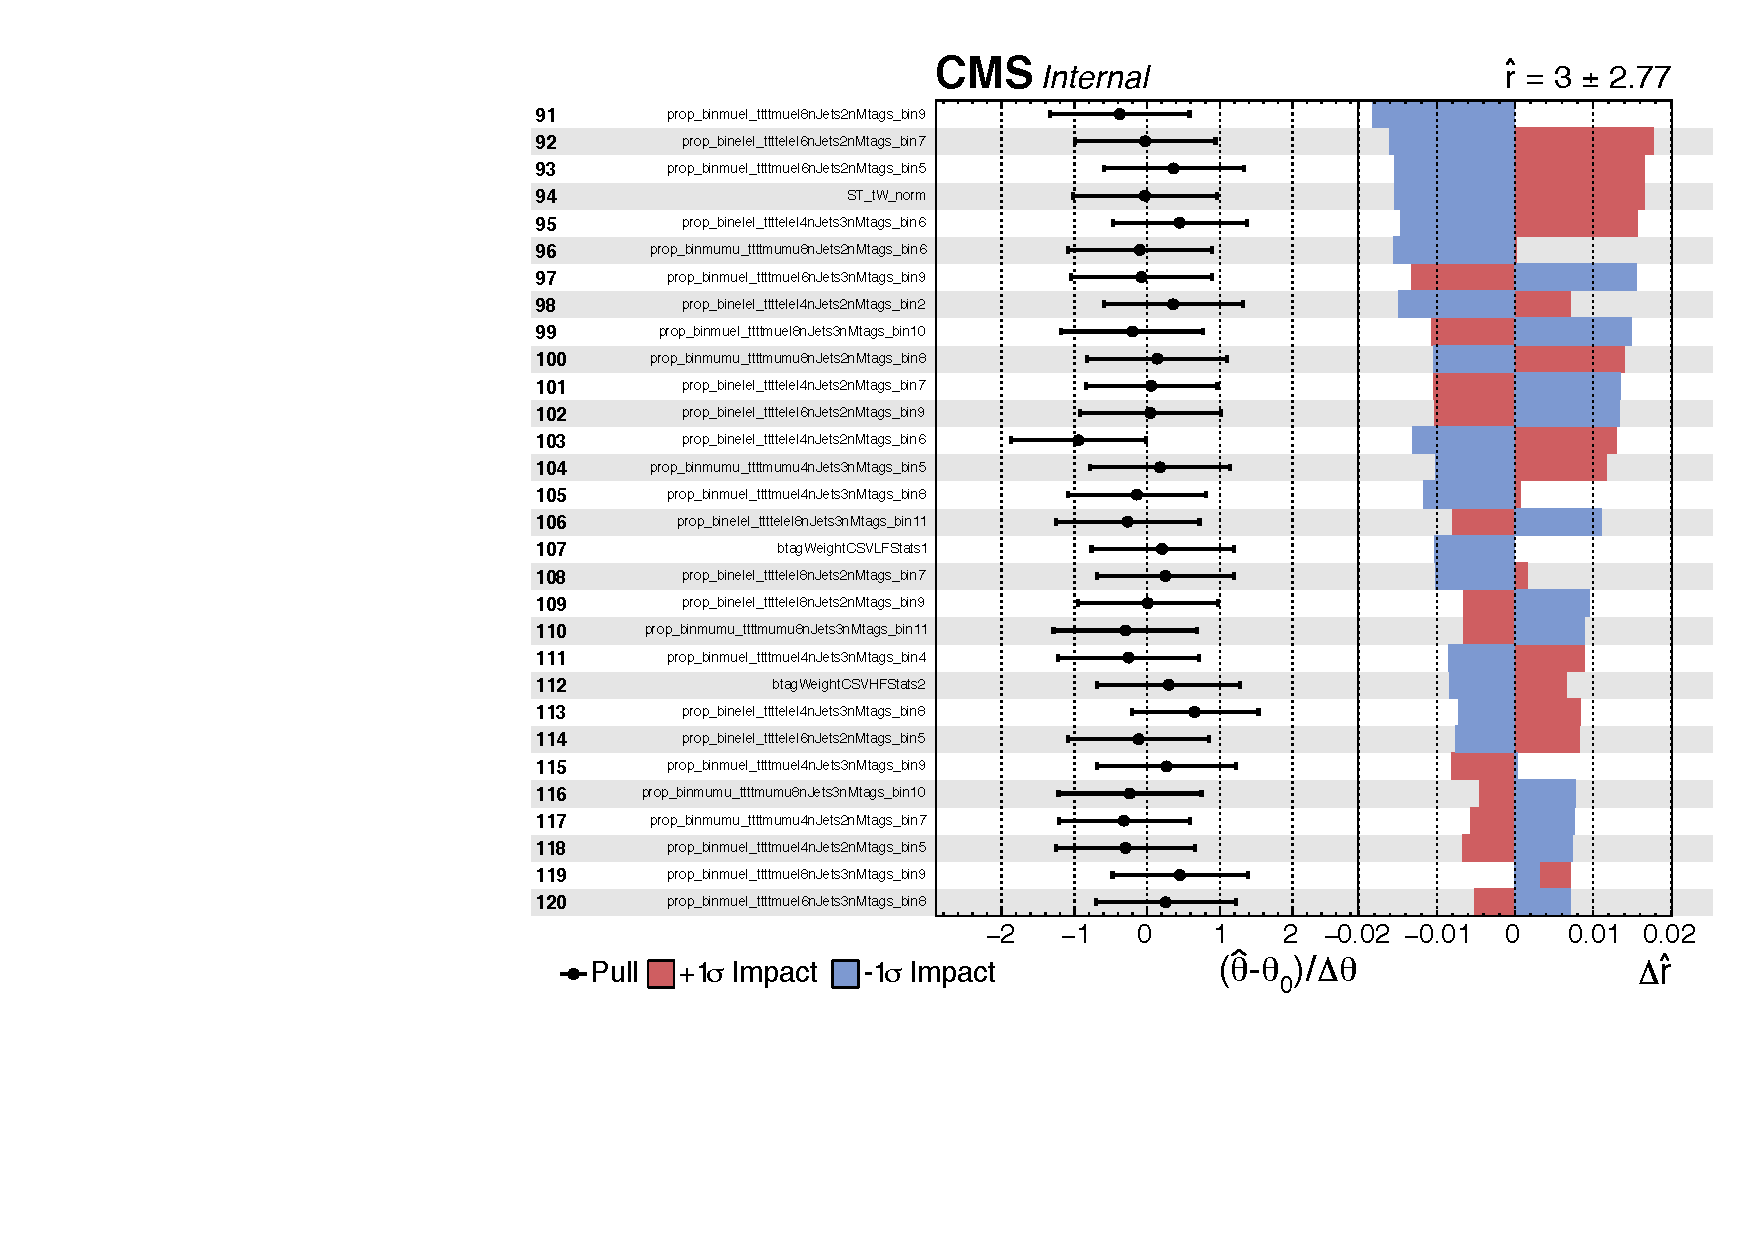
\includegraphics[width=0.45\textwidth]{impacts4.pdf}
\end{figure}
\end{frame}

%------------------------------------------------


\begin{frame}[label=impacts2]
\frametitle{impacts of nuisance parameters}
\vspace{-10pt}
\begin{columns}
	\column{0.5\textwidth}
	\begin{figure}
		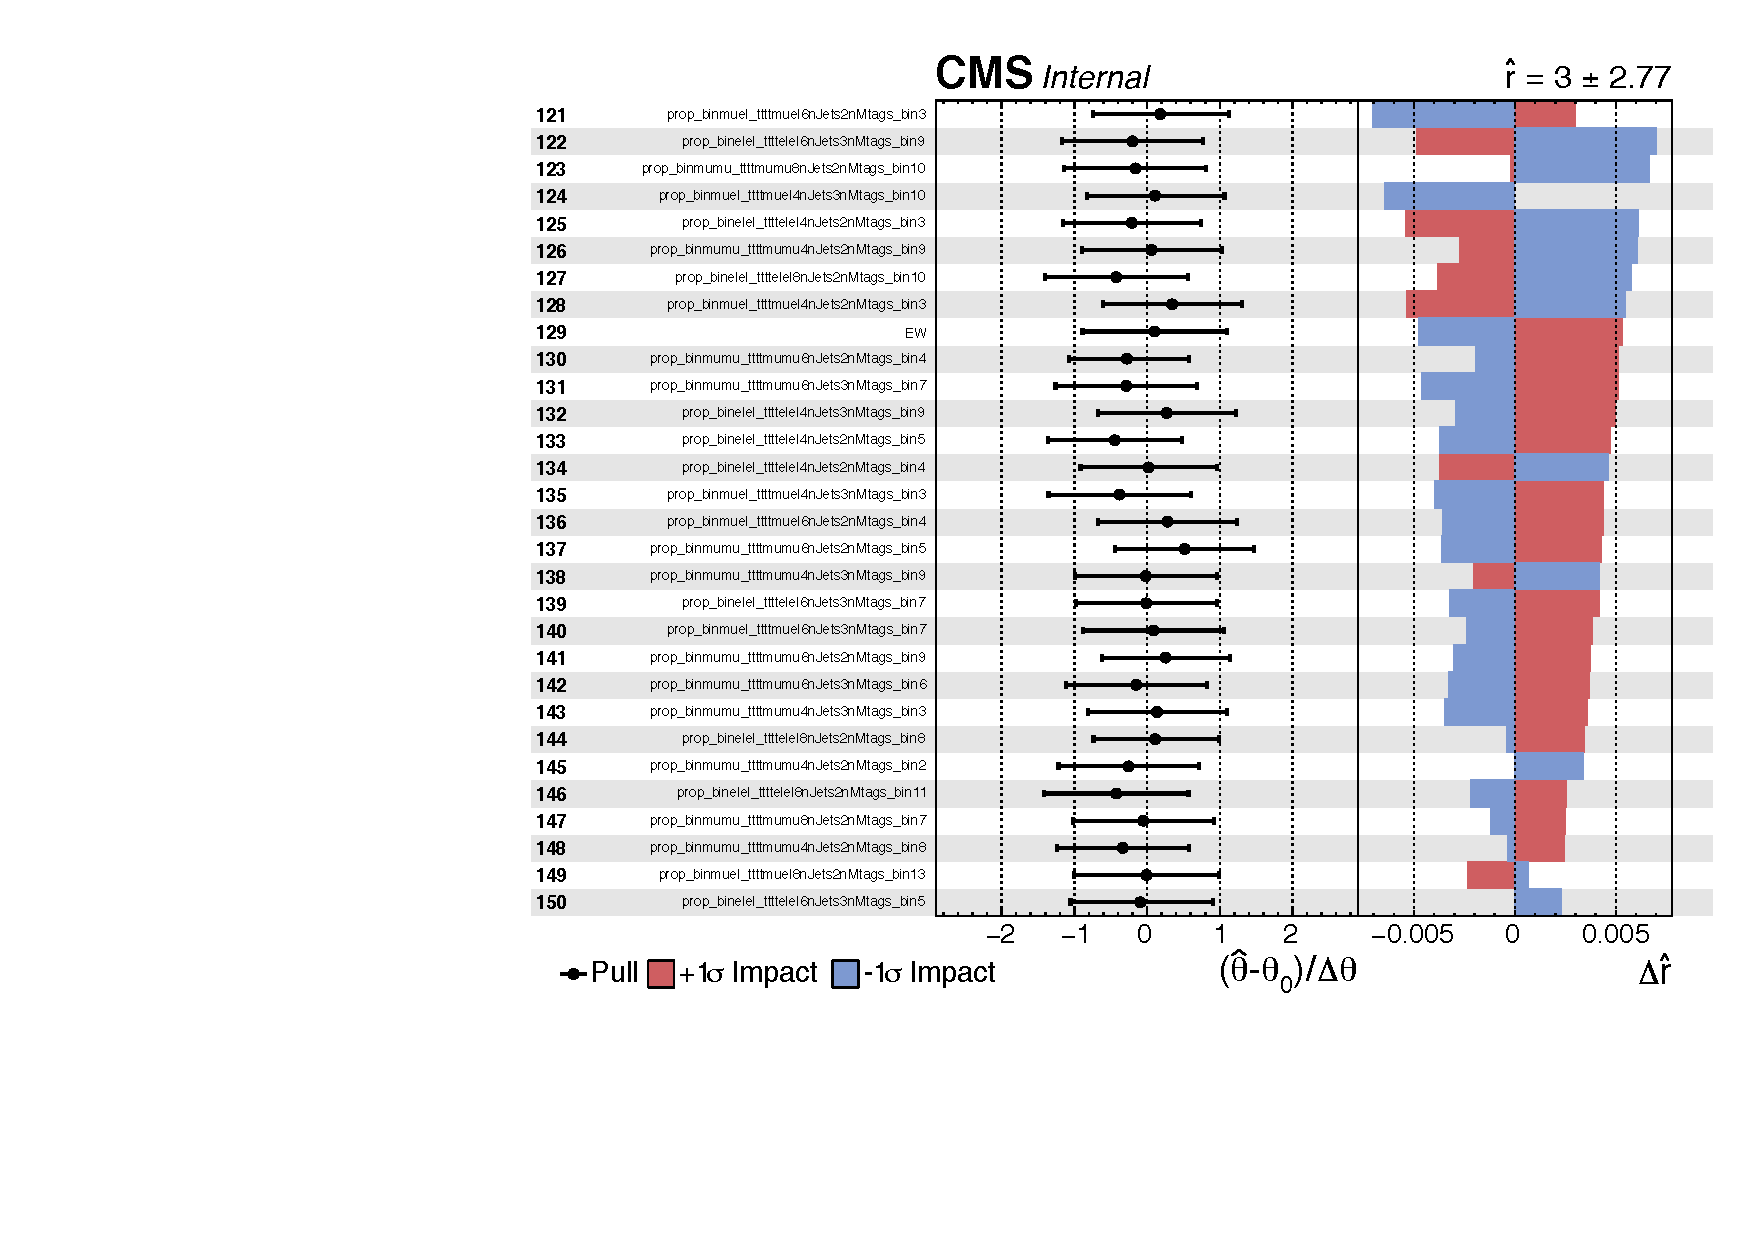
\includegraphics[width=0.9\textwidth]{impacts5.pdf}
	\end{figure}
	\column{0.5\textwidth}
	\begin{figure}
		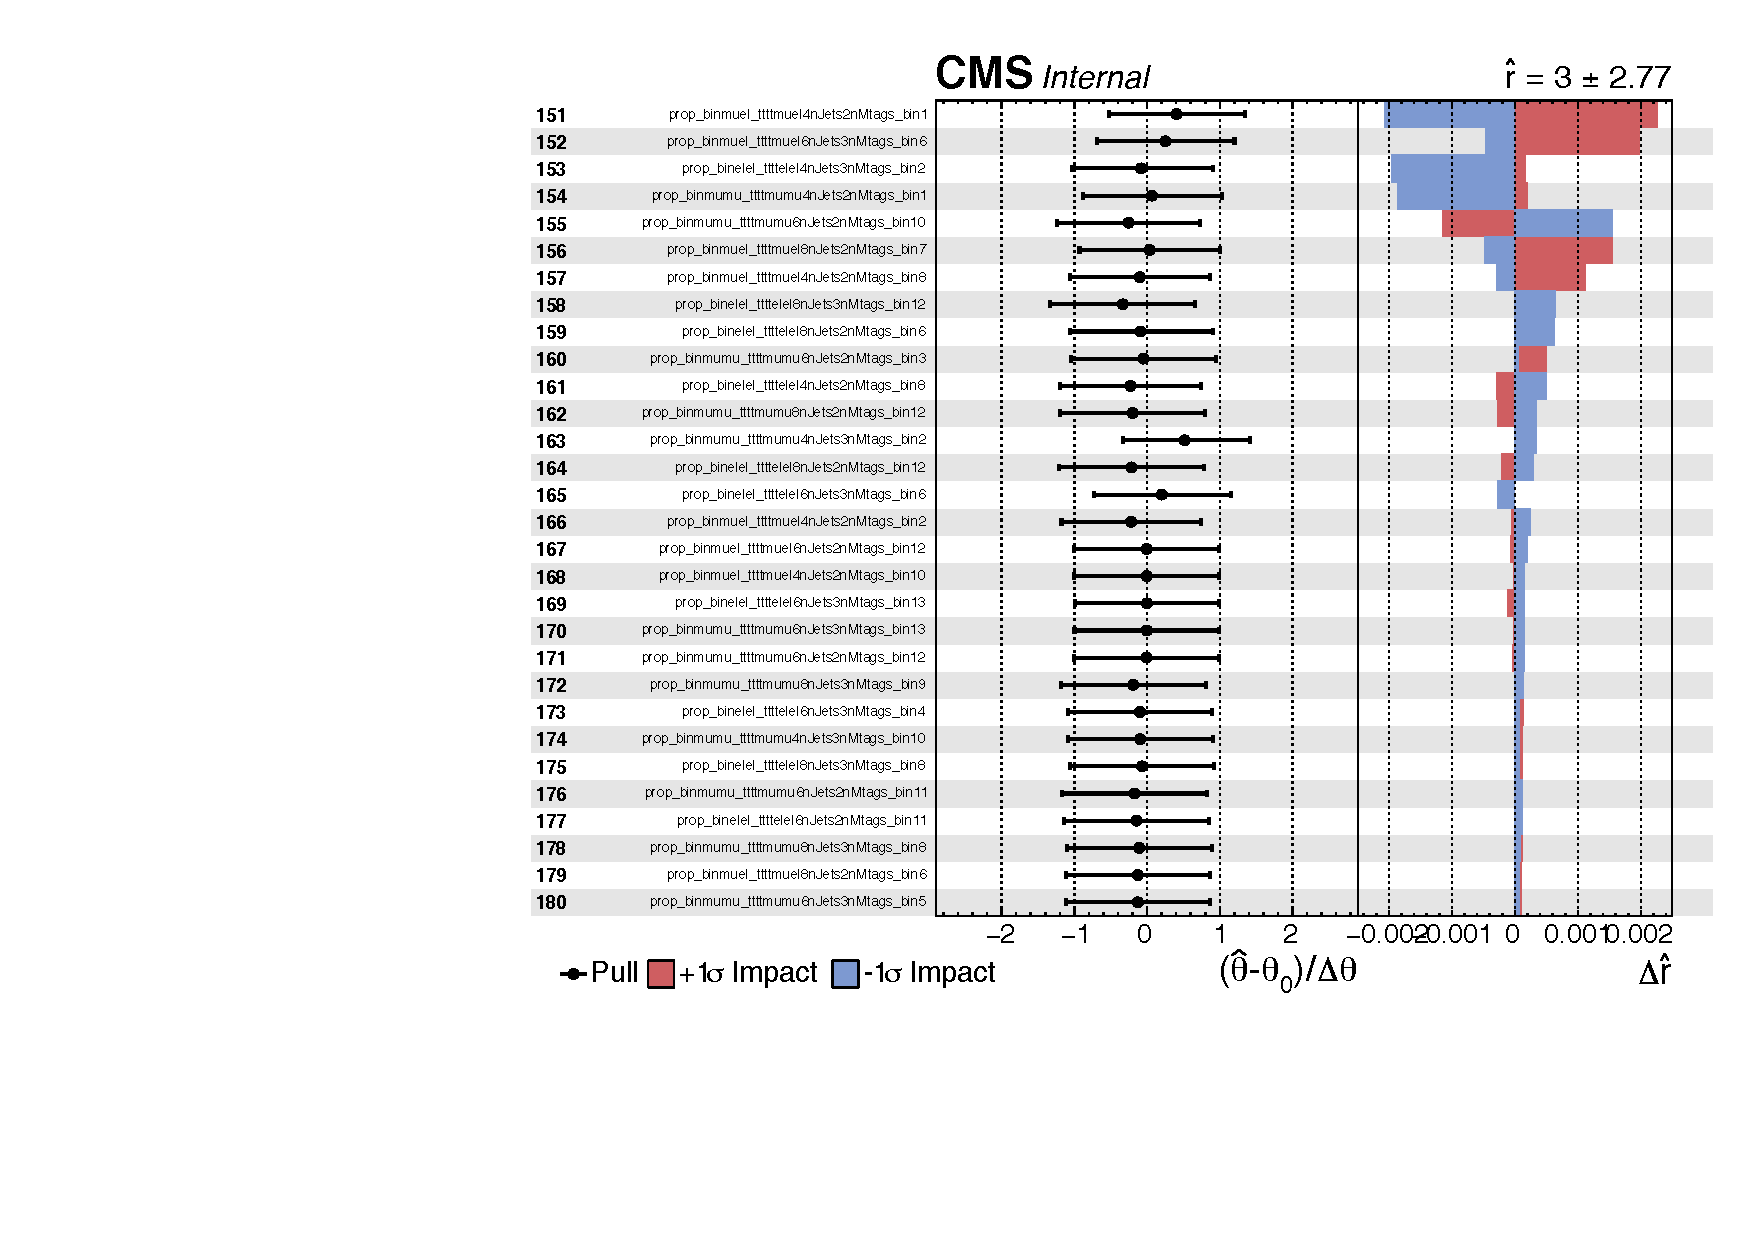
\includegraphics[width=0.9\textwidth]{impacts6.pdf}
	\end{figure}
\end{columns}
\vspace{-10pt}
\begin{figure}
	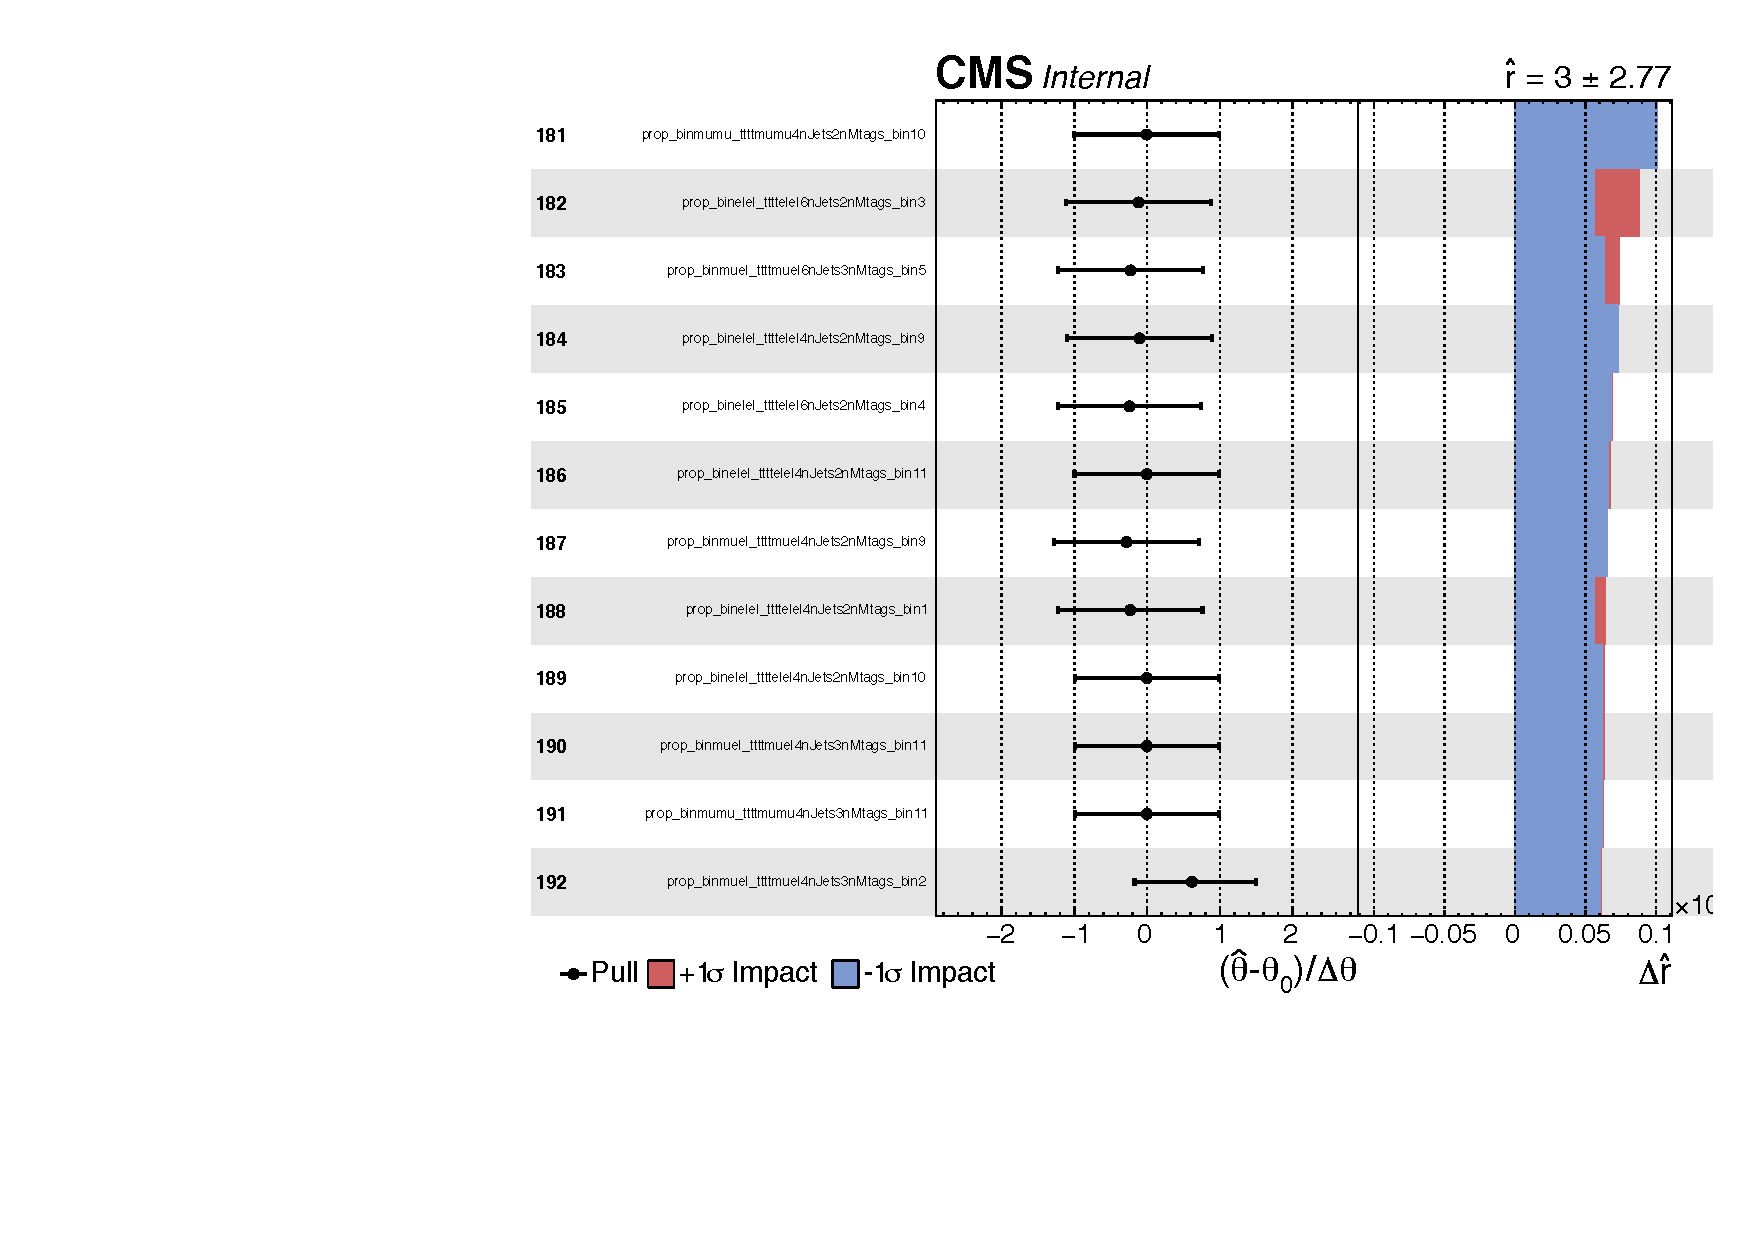
\includegraphics[width=0.45\textwidth]{impacts7.pdf}
\end{figure}\end{frame}

%------------------------------------------------

\begin{frame}
\frametitle{Maybe some more control plots?}
%\begin{figure}
%\includegraphics[width=0.8\linewidth]{test}
%\end{figure}
\end{frame}

%------------------------------------------------


%----------------------------------------------------------------------------------------

\end{document} 